\setcounter{chapter}{6}

\chapter{Neural Networks}

    The tools we've developed so far are interesting, and \textbf{varied}. We've discussed:
    
    \begin{itemize}
        \item \textbf{Regression}: the problem of creating \textbf{real-number} outputs based on data.
        \item \textbf{Classification}: the problem of \textbf{sorting} data points into \textbf{categories}.
        \item Gradient \textbf{descent}: A technique for gradually \textbf{improving} your model using \textbf{calculus}.
    \end{itemize}
    
    These concepts are fascinating in their own right, and can be used to handle some \textbf{simple} problems. But, when they are \textbf{combined} together, we get something much more \textbf{powerful}: \textbf{neural networks}.
    
    \subsection{Machine Learning Applications}
            
        Neural networks in the modern area are used to tackle complex and challenging problems:
        
        \begin{itemize}
            \item Image labelling and generation
                \begin{itemize}
                    \item \miniex \textbf{Recognizing} a \textbf{picture} of a dog. Or, \textbf{creating} a picture of a dog when prompted.
                \end{itemize}
            \item Physics simulation
                \begin{itemize}
                    \item \miniex \textbf{Simulating} water flow realistically, or special-effects smoke for a \textbf{movie}.
                \end{itemize}
            \item Financial prediction
                \begin{itemize}
                    \item \miniex Predicting how the \textbf{market} moves over time, and what the best \textbf{financial} choices in the present are.
                \end{itemize}
            \item Text processing and generation
                \begin{itemize}
                    \item \miniex Creating machines that can understand human text \textbf{prompts}, and writing useful \textbf{explanations} for humans.
                \end{itemize}
            \item Data analysis
                \begin{itemize}
                    \item \miniex \textbf{Compressing} data, or processing it to isolate the \textbf{important} aspects, without the noise.
                \end{itemize}
        \end{itemize}
        
        As you can see, \textbf{neural networks} are used in a wide array of very \textbf{difficult} problems. No wonder it's rapidly becoming so popular!
        
    \subsection{Neural Network Perspectives: The brain}
    
        So, what \textit{is} a neural network? Well, there's a \textbf{couple} ways of looking at it:
        
        First, the name comes from the fact that NNs are inspired by the \textbf{brain}: we call the basic units of a neural network a \textbf{neuron}.
        
        This gives us some general idea of the \textbf{structure} of a neural network:
        
        Just like in the \textbf{brain}, we take many individual units, called \textbf{neurons}, which we connect together to do more \textbf{complicated} tasks. That combined structure is a \textbf{neural network}.
            \note{Funny enough, as effective as neural networks are, we now think they don't work very much like the human brain! But we keep the terminology.}\\
        
        \begin{concept}
            \vocab{Neural networks} are inspired by the brain and its \purp{neurons}, in an effort to do better, \gren{human-like} computation.
            
            Based on this, neural networks are \purp{built} out of simple \gren{units} called \purp{neurons}, connected to each other.
        \end{concept}

        
    \subsection{Neural Network Perspectives: Classification and Regression}
    
        In this class, we \textbf{won't} focus on the brain analogy, though it did inspire the model.
        
        Instead, we will mostly think of \textbf{neural networks} in terms of what they're able to do, and how they work.
        
        One problem we have struggled with is certain tasks that can't be handled by \textbf{linear} models. We have used \textbf{feature representations} to work on this problem.
        
        Simply, some problems are outside our \textbf{hypothesis} space. But, there's another way: this is where \textbf{neural networks} come in.
        
        By combining lots of simple \textbf{units} ("neurons"), we can get a very \textbf{complex} model for solving our problems.
        
        With such a \textbf{rich} hypothesis class, combined with the power of \textbf{gradient descent}, we can create a model that can do \textbf{classification} or \textbf{regression} for very difficult problems!
            \note{Reminder: "richness" or "expressiveness" of a hypothesis reflect how wide our options are. Neural networks give us many possibilities for models. With more options, we can handle more problems!}\\
            
        \begin{concept}
            \vocab{Neural Networks} can create a very \vocab{rich hypothesis class} by combining many simple \gren{units}.
            
            With this \gren{hypothesis class}, we can handle \purp{regression} or \purp{classification} for very challenging \gren{problems}.
        \end{concept}
    
    \subsection{Building up a basic neural network}
        
        Let's make sense of what we said above, and \textbf{visualize} what a neural network might look like.
        
        We start with one function: a \textbf{neuron}. This function could be, for example, one we've used before: our logistic \textbf{classifier}, or linear \textbf{regression}. We'll ignore the details for now.
       
        \begin{figure}[H]
            \centering
            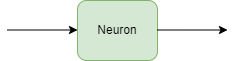
\includegraphics[width=60mm,scale=0.4]{images/nn_images/neuron.png}
        \end{figure}
       
        One neuron might not be very powerful, or \textbf{expressive}. It's useful, but limited. We've seen its weaknesses.
       
        We could try to use \textbf{feature transformations} to help us. But, let's think in a more \textbf{general} way: a transformation is just another \textbf{function} we apply to our input!
       
        \begin{figure}[H]
            \centering
            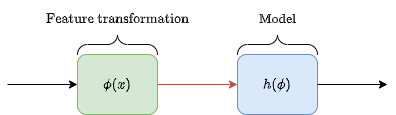
\includegraphics[width=80mm,scale=0.4]{images/nn_images/feature_transform.png}
        \end{figure}
       
        This gives us an \textbf{idea}: rather than trying to think of a single, more \textbf{complex} model, we could \textbf{combine} multiple simple models!
            \note{Note that feature transformations are a bit complex for what we'd usually put in a neuron. But, it gives us the right inspiration.}
       
        \begin{figure}[H]
        \centering
            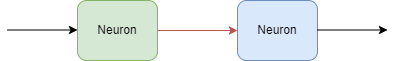
\includegraphics[width=80mm,scale=0.4]{images/nn_images/two_neurons.png}
        \end{figure}
        
        We could repeatedly add more neurons in \textbf{series}: each one being the input to another. And we'll do that later!
        
        But, there's another type of \textbf{complexity} we haven't explored: we could have two neurons in \textbf{parallel}.
            \note{This parallel/series vocabulary is borrowed from circuits. We'll just use it for demonstration: you don't need to remember it.}
        
        \begin{figure}[H]
        \centering
            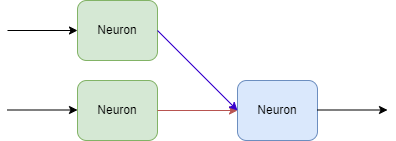
\includegraphics[width=100mm,scale=0.4]{images/nn_images/three_neurons.png}
        \end{figure}
        
        Now, we have \textbf{two} neurons feeding into one output neuron! This already looks like a more \textbf{complicated} model. 
        
        We can go even further: what if we have two outputs as well?
        
        \begin{figure}[H]
        \centering
            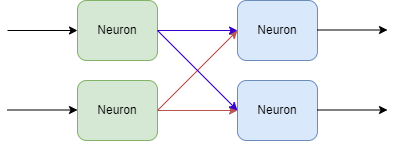
\includegraphics[width=100mm,scale=0.4]{images/nn_images/four_neurons.png}
        \end{figure}
        
        Because we had two \textbf{inputs}, we had to add two new \textbf{links} when we added the output neuron. This is getting difficult to \textbf{view}!
        
        We'll stop here for now, but you can imagine repeatedly \textbf{adding} more neurons in \textbf{parallel} (with the same inputs/outputs) or in \textbf{series} (as an input or output).
        
        And we each addition, the function gets more and more \textbf{complex}: you can create a \textbf{richer} hypothesis class!
        
        We'll explore how to do this \textbf{systematically} later in the chapter.
            \note{By "systematic", we just mean "in a way that's consistent and makes sense".}\\
        
        \begin{definition}
            \vocab{Neural Networks} are a \purp{class} of models that can be used to solve \gren{classification}, \gren{regression}, or other interesting problems.
            
            They create very \purp{rich} hypothesis classes by combining many \gren{simple} models, called \vocab{neurons}, into a \gren{complex} model.
            
            We do this combination \purp{systematically}, so that it is easy to \gren{analyze} and work with our \purp{model}.
            
            This creates a very \purp{flexible} hypothesis, which can be \gren{broken down} into its \purp{simple} parts and what \gren{connects} them.
        \end{definition}
        
    \subsection{Neural Network Perspectives: Predictions with Big Data}
    
        Our last major \textbf{perspective} on neural networks is one that you see in lots of modern \textbf{applications}. We won't work much with this perspective in this \textbf{class}, but our techniques \textbf{enable} it.
        
        Neural networks, because they can create such \textbf{sophisticated} models, can be used for problems in very \textbf{complex} domains: the kind of \textbf{applications} we discussed at the beginning of this chapter.
        
        These applications require a lot of \textbf{data} to build a good \textbf{model}, however. So, machine learning models often take \textbf{huge} amounts of data, with lots of energy and time to train them.
        
        But, once they are fully \textbf{trained}, they can give predictions very \textbf{quickly}, and often very \textbf{accurately}.\\
        
        \begin{concept}
            \vocab{Neural networks} can be seen as a way to make \purp{predictions} based on huge amount of \gren{data} for very \purp{complex} problems.
        \end{concept}
        

\section{Basic Element}

    Now, we have idea of what neural networks \textbf{are}. But, we have yet to handle the \textbf{details}:
    
    \begin{itemize}
        \item What \textbf{is} a neuron?
        \item How do we "systematically" \textbf{combine} our neurons?
        \item How do we \textbf{train} this, like we would a \textbf{simple} model?
    \end{itemize}
    
    We'll handle all of these steps and more - the above description was just to give a \textbf{high-level} view of what we want to \textbf{accomplish}. 
    
    Now, we go down to the \textbf{bottom} level, and think about just \textbf{one neuron}: what does it look like, and how does it work?
    
    First, some terminology:\\
    
    \begin{notation}
        \vocab{Neurons} are also sometimes called \vocab{units} or \vocab{nodes}.
        
        They are mostly \gren{equivalent} names. They just reflect different \purp{perspectives}.
    \end{notation}
    
    \subsection{What's in a neuron: The Linear Component}
    
        As we mentioned before, our goal is to combine \textbf{simple} units into a \textbf{bigger} one. So, we want a model that's \textbf{simple}.
        
        Well, let's start with what we've done before: we've worked with the \textbf{linear} model
        
        \begin{equation}
            h(x) = \theta^T x + \theta_0
        \end{equation}
        
        This model has lots of nice properties:
        
        \begin{itemize}
            \item It limits itself to \textbf{addition} and \textbf{multiplication} (easy to compute)
            
            \item \textbf{Linearity} lets us prove some mathematical things, and use vector/\textbf{matrix} math
            
            \item The dot product between $\theta$ and $x$ has a nice \textbf{geometric} interpretation.
        \end{itemize}
        
        This will make up the \textbf{first} part of our model.\\
        
        \begin{concept}
            Our \vocab{neuron} contains a \purp{linear} function as its \gren{first} component.
        \end{concept}
    
    \subsection{Weights and Biases}
    
        But, there's one minor \textbf{change}: before, we used $\theta$ because it represented our \textbf{hypothesis}. 
        
        But, every neuron is going to have its own \textbf{values} for its \textbf{linear} model:
        
        \begin{equation}
            \overbrace{
                f_1(x)
            }^{\text{Neuron 1}}
            = Ax+B 
            \qquad \qquad \qquad
            \overbrace{
                f_1(x)
            }^{\text{Neuron 2}}
            = Cx+D
        \end{equation}
        
        It wouldn't make much \textbf{sense} to call both $A$ and $C$ by the name $\theta$. 
        
        We could use some clever \textbf{notation}, but why treat them as \textbf{hypotheses}? They are each only a \textbf{part} of our hypothesis $\Theta$.
        
        So, instead of thinking of each as a "hypothesis", let's switch perspectives.
        
        Each value $\theta_k$ \textbf{scales} how much $x_k$ affects the \textbf{output}: if we're doing
        
        \begin{equation}
            g(x) = 100x_1+2x_2
        \end{equation}
        
        Then, changing $x_1$ will have a much \textbf{bigger} effect on $g(x)$. Another way to say this is it \textbf{weighs} more heavily: it matters \textbf{more}.
        
        Because of that, we call the number we scale $x_1$ by a \textbf{weight}.\\
        
        \begin{notation}
            A \vocab{weight} $w_k$ tells you how heavily a \purp{variable} $x_k$ \gren{weighs} into the output.
            
            $w_k$ is \purp{equivalent} to $\theta_k$: it's a \gren{scalar} $w_k \in \RR$.
            
            \begin{equation*}
                \Big( 
                    \red{\theta_1}x_1 + \blu{\theta_2}x_2 
                \Big)
                \Longleftrightarrow 
                \Big(
                    \red{w_1}x_1+\blu{w_2}x_2
                \Big)
            \end{equation*}
            
            We can combine it into a vector $w \in \RR^m$.
            
            \begin{equation*}
                w = 
                    \begin{bmatrix}
                      w_1 \\ w_2 \\ \vdots \\ w_m
                    \end{bmatrix}
                \qquad \qquad \qquad
                \theta^Tx \Longleftrightarrow w^Tx
            \end{equation*}
        \end{notation}
        
            \note{Remember that $a \Longleftrightarrow b$ means $a$ and $b$ are equivalent!} 
        
        
        What about our other term, $\theta_0$? We call it an \textbf{offset}: it's the value we \textbf{shift} our linear model away from \textbf{origin}.
        
        We'll use the same notation:\\
        
        \begin{notation}
            An \vocab{offset} $w_0$ tells you how far we \purp{shift} $h(x)$ away from the origin. 
            
            $w_0$ is \purp{equivalent} to $\theta_0$: it's a \gren{scalar} $w_0 \in \RR$
            
            \begin{equation*}
                \Big(
                    (\theta^Tx) + \red{\theta_0} 
                \Big)
                \Longleftrightarrow 
                \Big(
                    (w^Tx) + \red{w_0}
                \Big)
            \end{equation*}
            
            We also sometimes call this the \vocab{threshold} or the \vocab{bias}.
        \end{notation}
        
        This gives us our linear model using our new notation:\\
        
        \begin{definition}
            The \vocab{linear component} for a neuron is given by
            
            \begin{equation*}
                z(x) = w^Tx + w_0
            \end{equation*}
            
            where $w \in \RR^m$ and $w_0 \in \RR$.
            
            \begin{equation*}
                w = 
                    \begin{bmatrix}
                      w_1 \\ w_2 \\ \vdots \\ w_m
                    \end{bmatrix}
            \end{equation*}
        \end{definition}
    
    \subsection{Linear Diagram}
    
        Now, we want to be able to depict our \textbf{linear} subunit. Let's do it piece-by-piece.
        
        First, we have our vector $\blu{x} = [x_1, x_2, ..., x_m]^T$:
        
        \begin{figure}[H]
            \centering
            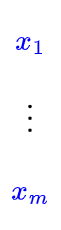
\includegraphics[width=10mm,scale=0.4]{images/nn_images/x_vector.png}
        \end{figure}
        
        Now, we want to \textbf{multiply} each term $x_i$ by its corresponding \textbf{weight} $w_i$. We'll combine them into a \textbf{function}:
        
        
        \begin{figure}[H]
            \centering
            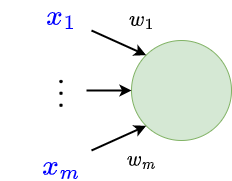
\includegraphics[width=30mm,scale=0.4]{images/nn_images/weights.png}
            \caption*{The circle represents our function.}
        \end{figure}
        
        How are we combining them? Well, we're adding them together.
        
        \begin{figure}[H]
            \centering
            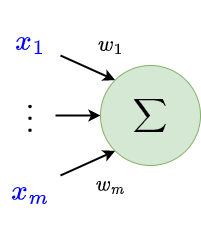
\includegraphics[width=25mm,scale=0.4]{images/nn_images/sigma.png}
        \end{figure}
        
        Note that we use the $\sum$ symbol, because we're \textbf{adding} after we \textbf{multiply}. In fact, we can write this as
        
        \begin{equation}
            w^T \blu{x} = \sum_{i=1}^m w_i\blu{x_i}
        \end{equation}
        
        We'll include the bias term as well: remember that we can represent $w_0$ as $1 * w_0$ to match with the other terms.
        
        \begin{figure}[H]
            \centering
            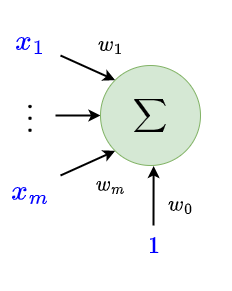
\includegraphics[width=30mm,scale=0.4]{images/nn_images/bias.png}
            \caption*{The blue "1" term is \textbf{multiplied} by $w_0$, just like how $x_k$ gets multiplied by $w_k$.}
        \end{figure}
        
        We have our full function! All we need to do is include our output, $\red{z}$:\\
        
        \begin{notation}
            We can depict our linear function $\red{z} = w^T\blu{x}+w_0$ as
            \begin{figure}[H]
            \centering
            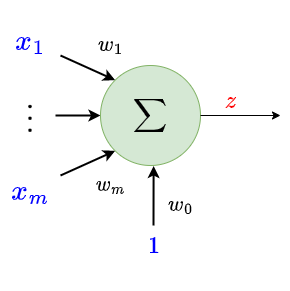
\includegraphics[width=40mm,scale=0.4]{images/nn_images/linear_subunit.png}
        \end{figure}
        \end{notation}
        
        Thus, $z$ is a function of $x$:
        
        \begin{equation}
            \red{z}(\blu{x}) = w^T\blu{x}+w_0
        \end{equation}
        
        Which, in $\sum$ notation, we could write as
        
        \begin{equation}
            \red{z}(\blu{x}) = \Bigg( \sum_{i=1}^m w_i\blu{x_i} \Bigg) +w_0
        \end{equation}
        
    \subsection{Adding nonlinearity}
    
        We'll continue building our neuron based on what we've done \textbf{before}. When doing linear regression, that linear unit was all we had. 
        
        But, once we do classification, we found that it was helpful to have a second, \textbf{non-linear} component: we used \textbf{sigmoid} $\sigma(u)$.
        
        We might not necessarily want the \textbf{same} nonlinear function, so instead, we'll just generalize: we have \textit{some} second component, which is allowed to be \textbf{nonlinear}.
        
        We call this component our \textbf{activation} function. Why do we call it that? It comes from the historical \textbf{inspiration} of neurons in the brain.
        
        Biological neurons only "fire" (give an output) above a certain threshold of \textbf{input}: that's when they \textbf{activate}.
            \note{Some activation functions reflect this, but they don't have to.}\\
            
        \begin{definition}
            Our \vocab{neuron} contains a potentially \purp{nonlinear} function $f$ called an \vocab{activation function} as its \gren{second} component.
            
            We notate this as 
            
            \begin{equation}
                \pur{a} = f(\red{z})
            \end{equation}
            
            Where $z$ is the \gren{output} of the \purp{linear} component, and $a$ is the \gren{output} of the \purp{activation} component.
            
            Note that $z$ and $a$ are \purp{real numbers}: we have $f: \RR \rightarrow \RR$
            
        \end{definition}
    
    \subsection{Nonlinear Diagram}
    
        We'll depict a function $f$.

        \begin{figure}[H]
            \centering
            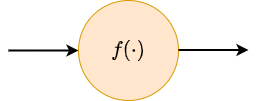
\includegraphics[width=40mm,scale=0.4]{images/nn_images/nonlinear_func.png}
        \end{figure}
        
        It takes in our \textbf{linear} output, $\red{z}$, and outputs our \textbf{neuron} output, $\pur{a}$.
        
        \begin{figure}[H]
            \centering
            \qquad\quad\;
            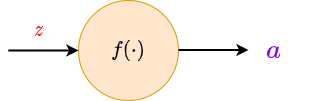
\includegraphics[width=60mm,scale=0.4]{images/nn_images/nonlinear_unit.png}
        \end{figure}
        
        Note some vocabulary used for $z$:\\
        
        \begin{notation}
            $z$, the \purp{output} of our \gren{linear} function, is called the \vocab{pre-activation}.
            
            This is because it is the result \purp{before} we run the \gren{activation} function.
        \end{notation}
        
        And for $a$:\\

        \begin{notation}
            $a$, the \purp{output} of our \gren{activation} function, is called the \vocab{activation}.
        \end{notation}
        
    \subsection{Putting it together}
    
        So now, our neuron is complete.\\

        \begin{definition}
            Our \vocab{neuron} is made of 
            
            \begin{itemize}
                \item A \vocab{linear} component that takes the neuron's input \blu{$x$}, and applies a linear function  
                
                    \begin{equation*}
                        \red{z} = w^T \blu{x} + w_0
                    \end{equation*}
                    
                    \begin{itemize}
                        \item The \vocab{pre-activation} $\red{z}$ is the \purp{output} of the \purp{linear} function.
                        \item It is also the \gren{input} of the \gren{activation function} $f$.
                    \end{itemize}
                    
                \item A (potentially nonlinear) \vocab{activation} component that takes the pre-activation $\red{z}$ and applies an \vocab{activation function} $f$:
                
                    \begin{equation*}
                        \pur{a} = f(\red{z})
                    \end{equation*}
                    
                    \begin{itemize}
                        \item The \vocab{activation} $\pur{a}$ is the \purp{output} of this \purp{activation function}.
                    \end{itemize}
            \end{itemize}
            
            When we \purp{compose} them together, we get
            
            \begin{equation*}
                \pur{a} = f(\red{z}) = f \Big(  w^T \blu{x} + w_0 \Big)
            \end{equation*}
            
        \end{definition}
        
            \note{When we say "compose", we mean \textbf{function composition}: combining $f(x)$ and $g(x)$ into $f(g(x))$.}
        
        We can also use $\sum$ notation to get:
        
        \begin{equation*}
            \pur{a} = f(\red{z}) = 
            f 
            \Bigg(
                \bigg( 
                    \sum_{i=1}^m w_i\blu{x_i} 
                \bigg) 
                + w_0 
            \Bigg)
        \end{equation*}
        
    \subsection{Neuron Diagram}
    
        Finally, we can \textbf{compose} our neuron into one big \textbf{diagram}:
        
        \begin{figure}[H]
            \centering
            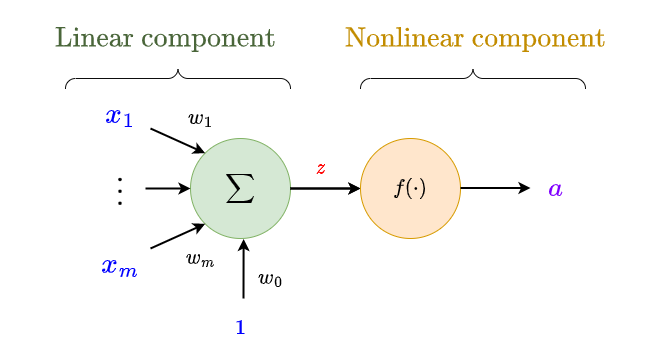
\includegraphics[width=100mm,scale=0.4]{images/nn_images/labelled_neuron.png}
        \end{figure}
        
        From here on out, we'll treat this as a \textbf{single} object:
        
        \begin{figure}[H]
            \centering
            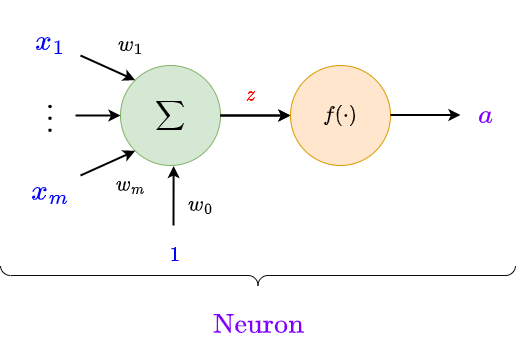
\includegraphics[width=80mm,scale=0.4]{images/nn_images/neuron_underbrace.png}
        \end{figure}
        
        \begin{notation}
            We can depict our \vocab{neuron} $f(w^T\blu{x}+w_0)$ as
            
            \begin{figure}[H]
                \centering
                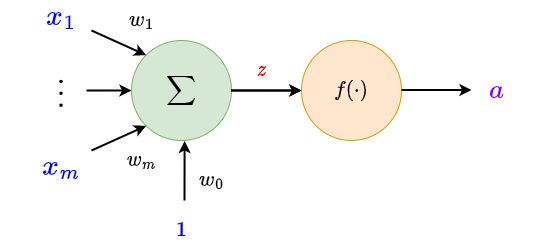
\includegraphics[width=100mm,scale=0.4]{images/nn_images/full_neuron.png}
            \end{figure}
            
            \begin{itemize}
                \item $x$ is our \gren{input} (neuron input, linear input )
                
                \item $z$ is our \purp{pre-activation} (linear output, activation input)
                
                \item $a$ is our \purp{activation} (neuron output, activation output)
            \end{itemize}
        \end{notation}
    
        This neuron will be the \textbf{basic unit} we work with for the rest of this \textbf{chapter} - it's one of the most \textbf{important} objects in all of machine learning.
        
    \subsection{Our Loss Function}
    
        One more detail: we will want to \textbf{train} these neurons. In order to be able to \textbf{measure} their performance, we'll need a \textbf{loss} function.
        
        This \textbf{isn't} any different from usual: we just need a \textbf{function} of the form
        
        \begin{equation}
            \loss(g,y)
        \end{equation}
        
        In \textbf{regression}, we wrote our loss as
        
        \begin{equation*}
            \loss 
            \Big( \;\;
                \blu{h(x; \Theta)}, \;\;
                \red{y} 
            \;\;\Big) 
        \end{equation*}
        
        The right term, $\eyi$, is unchanged: we still need to compare against the \textbf{correct} answer.
        
        The main change is we aren't using $\Theta$ notation: we'll \textbf{replace} it with $(w,w_0)$
        
        \begin{equation*}
            \loss 
            \Bigg( \;\;
                h
                \Big(
                    x; \pur{(w, w_0)}
                \Big), \;\;
                y 
            \;\;\Bigg) 
        \end{equation*}
        
        And finally, we get the loss for multiple data points: 
            \note{We skip doing $1/n$ averaging because we often use this for SGD: we plan to take small steps as we go, rather than adding up our steps all at once.}
        \begin{equation*}
            \sum_i
            \loss 
            \Bigg( \;\;
                h
                \Big(
                    \blu{\exi}; (w, w_0)
                \Big), \;\;
                \blu{\eyi} 
            \;\;\Bigg) 
        \end{equation*}
        
        And with this, not only is our neuron \textbf{complete}, but we have everything we need to \textbf{work} with it.\\
        
        \begin{concept}
            For a \vocab{complete neuron}, we need to specify
        
            \begin{itemize}
                \item Our \purp{weights} and \gren{offset}
                \item Our \purp{activation} function
                \item Our \purp{loss} function
            \end{itemize}
        \end{concept}
        
        From here, we could do \textbf{stochastic gradient descent} as we usually do, to \textbf{optimize} this neuron's \textbf{performance}.
        
    \subsection{Example: Linear Regression}
    
        Let's go through some \textbf{examples}. We mentioned in the \textbf{beginning} of this chapter that our neuron could be most of the simple \textbf{models} we've worked with.
        
        So, let's give that a go: we'll start by doing \textbf{linear regression}.
        
        \begin{equation*}
            h(x) = \theta^T x + \theta_0
        \end{equation*}
        
        This model is exclusively \textbf{linear}: we just have to replace $\theta$ with $w$.
        
        \begin{equation*}
            \red{z}(x) = w^T x + w_0
        \end{equation*}
        
        So, our linear component is \textbf{done}: $(\theta, \theta_0) = (w, w_0)$.
        
        What about our \textbf{activation} function?
        
        Well, activation allows for \textbf{nonlinear} functions. But, we don't \textbf{want} to make it nonlinear. 
        
        In fact, we've already got what we \textbf{want}: we don't want the \textbf{activation} to do anything at \textbf{all}.
        
        So, we'll use \textbf{this} function:\\
        
        \begin{concept}
            The \vocab{identity function} $f(z)$ is a function that has no \gren{effect} on your \purp{input}.
            
            \begin{equation*}
                f(\red{z}) = \red{z}
            \end{equation*}
            
            By "having no effect", we mean that the input is \purp{unchanged}: this is true even if your input is \gren{another function}:
            
            \begin{equation}
                f(g(x)) = g(x)
            \end{equation}
        \end{concept}
        
            \note{We call it the "identity" because the input's identity is unchanged!}
        
        So, the \textbf{identity} function is our activation function: it keeps our \textbf{linearity}.\\
        
        \begin{concept}
            \vocab{Linear Regression} can be represented with a \gren{single neuron} where
            
            \begin{itemize}
                \item We keep our \purp{linear component}, but set $(\theta, \theta_0) = (w, w_0)$.
                
                \begin{equation*}
                    \red{z}(x) = w^Tx+w_0
                \end{equation*}
                
                \item Our \purp{activation function} is the \gren{identity} function, 
                
                \begin{equation*}
                    f(\red{z}) = \red{z}
                \end{equation*}
                
                \item Our \purp{loss function} is \gren{quadratic loss}.
                
                \begin{equation*}
                    \loss(\pur{a},y) = (\pur{a}-y)^2
                \end{equation*}
                
            \end{itemize}
        \end{concept}
        
        \begin{figure}[H]
            \centering
            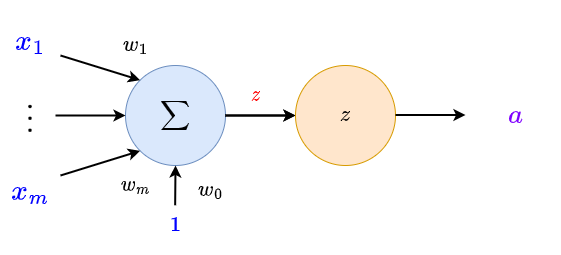
\includegraphics[width=100mm,scale=0.4]{images/nn_images/linear_reg.png}
        \end{figure}
    
    \subsection{Example: Linear Logistic Classifiers}
    
        Now, we do the same for LLCs: it's already broken up into \textbf{two} parts in our \textbf{classification} chapter.
        
        First, the \textbf{linear} component. This is the same as linear regression:
        
        \begin{equation}
            \red{z} = 
            \theta^T x + \theta_0
        \end{equation}
        
        And then, the \textbf{logistic} component:
        
        \begin{equation}
            \sigma(\red{z}) = \frac{1}{1+e^{-\red{z}}}
        \end{equation}
        
        This second part is \textbf{nonlinear}: its our \textbf{activation} function!\\
        
        \begin{concept}
            A \vocab{Linear Logistic Classifier} can be represented with a \gren{single neuron} where
            
            \begin{itemize}
                \item We keep our \purp{linear component}, but set $(\theta, \theta_0) = (w, w_0)$.
                
                \begin{equation*}
                    \red{z}(x) = w^Tx+w_0
                \end{equation*}
                
                \item Our \purp{activation function} is the \gren{sigmoid} function, 
                
                \begin{equation*}
                    f(\red{z}) = \sigma(\red{z}) = \frac{1}{1+e^{-\red{z}}}
                \end{equation*}
                
                \item Our \purp{loss function} is \gren{negative-log likelihood} (NLL)
                
                \begin{equation*}
                    \loss_{nll}
                    (\pur{a} ,\quad \byi)
                    =
                    -
                    \Bigg(
                        \byi \log{\pur{a}}
                        +
                        \left( 1 - \byi \right)
                        \log
                        \left( 1-\pur{a} \right) 
                    \Bigg)
                \end{equation*}
            
            \end{itemize}
        \end{concept}
        
        \begin{figure}[H]
            \centering
            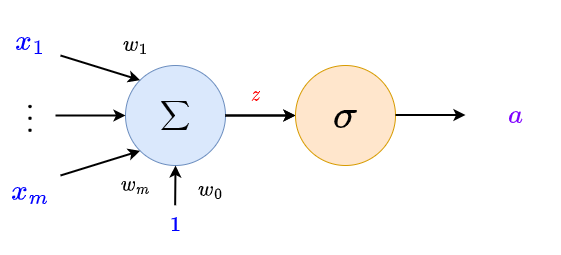
\includegraphics[width=100mm,scale=0.4]{images/nn_images/llc_unit.png}
        \end{figure}
        
\pagebreak
%%%%%%%%%%%%%%%%%%%%%%%%%%%%%%%%%%%%%%%%%%%%%%%%%%%%%%%%%%%%%%%%%%%%%%%%%%%%%    
    
\section{Networks}

    Now, we have fully developed the individual \textbf{neuron}. 
    
    We can even do \textbf{gradient descent} on it: just like when we were doing LLCs, we can use the \textbf{chain rule}. 
        \note{We'll get into this more, later in the chapter.}
        
    So, we return to the idea from the beginning of this chapter: combining multiple neurons into a \textbf{network}. 
    
    \subsection{Abstraction}
        For this next section, we'll \textbf{simplify} the above diagram to this:
        
        \begin{figure}[H]
            \centering
            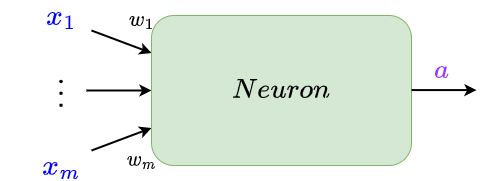
\includegraphics[width=60mm,scale=0.4]{images/nn_images/neuron_abstraction.png}
        \end{figure}
        
        In fact, for more \textbf{simplicity}, we'll draw \textbf{one} arrow to represent the whole vector $x$. However, nothing about the \textbf{actual} math has changed.
        
        \begin{figure}[H]
            \centering
            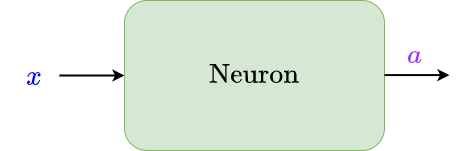
\includegraphics[width=50mm,scale=0.4]{images/nn_images/neuron_abstraction_x.png}
        \end{figure}
        
        This is also called \textbf{abstraction} - we need it a lot in this chapter.\\
        
        \begin{definition}
            \vocab{Abstraction} is a way to view your system more \gren{broadly}: removing excess details, to make it \gren{easier} to work with.
            
            Abstraction takes a \purp{complicated} system, and focuses on only the \purp{important} details. Everything else is \gren{excluded} from the model.
            
            Often, this \purp{simplified} view boils a system down to its the \gren{inputs} and \gren{outputs}: the "interface".
        \end{definition}
        
        \miniex Rather than thinking about all of the \textbf{mechanics} of how a car works, you might \textbf{abstract} it down to the pedals, the steering wheel, and how that causes the car to move.
    
    \subsection{Some limitations: acyclic networks}
    
        We won't allow for just \textbf{any} kind of network: we can create ones that might be unhelpful, or just very \textbf{difficult} to \textbf{analyze}. 
        
        For now, we can get interesting and \textbf{useful} behavior while keeping it \textbf{systematic}. We'll define this "system" later.
    
        We'll assume our networks are \textbf{acyclic}: they do not create closed \textbf{loops}, where something can affects it own input.
        
        \begin{figure}[H]
            \centering
            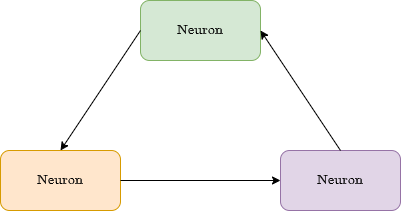
\includegraphics[width=100mm,scale=0.4]{images/nn_images/cyclic_network.png}
            \caption*{This is a cyclic network: this is messy and we won't worry about this for now.}
        \end{figure}
        
        This means information only \textbf{flows} in one direction, "forward": it never flows "backwards".\\
        
        \begin{concept}
            For simple \vocab{neural networks}, we assume that they are \purp{acyclic}: there are no \gren{cycles}, or loops.
            
            This means that \purp{no neuron} has an output that affects its \gren{input}, directly or indirectly.
            
            We call these \vocab{feed-forward} networks.
        \end{concept}
        
        We'll show how to build up the rest of what we need.
    
    \subsection{How to build networks}
        
        Suppose we have two neuron in \textbf{series}, our \textbf{simplest} arrangement:
        
        \begin{figure}[H]
            \centering
            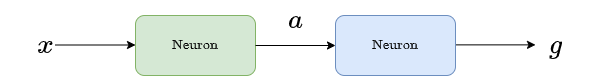
\includegraphics[width=100mm,scale=0.4]{images/nn_images/series_a.png}
        \end{figure}
        
        Our first neuron takes in a whole \textbf{vector} of values, $x = [x_1, x_2, ..., x_m]^T$. But, it only \textbf{outputs} a single value, $a$.
            \note{Remember that while we only see one arrow from $x$, each data point $x_i$ is included.}
        
        That means the second neuron only receives \textbf{one} value, but it's capable of handling a full \textbf{vector}. We can add more values!
        
        Let's add \textbf{another} neuron.
        
        \begin{figure}[H]
            \centering
            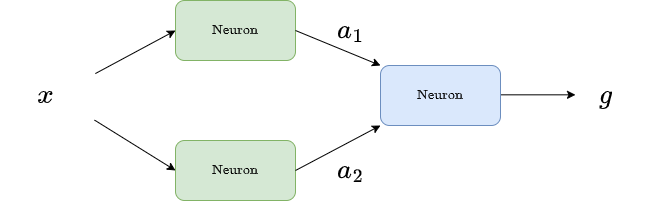
\includegraphics[width=100mm,scale=0.4]{images/nn_images/two_neurons_a.png}
        \end{figure}
        
        Our rightmost neuron now has \textbf{2 inputs}, which can be stored in a vector,
        
        \begin{equation}
            A = 
            \begin{bmatrix}
              a_1 \\ a_2
            \end{bmatrix}
        \end{equation}
        
        We could increase the \textbf{length} of this vector by adding more \textbf{neurons}.
        
        \begin{figure}[H]
            \centering
            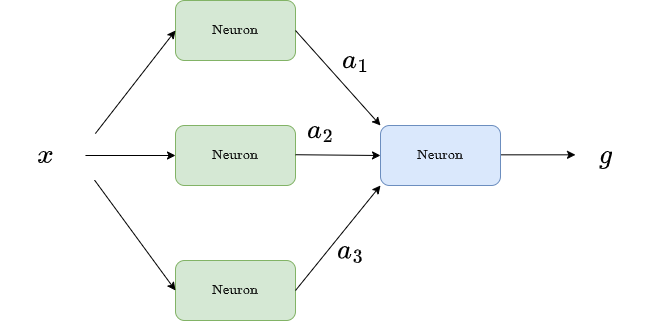
\includegraphics[width=100mm,scale=0.4]{images/nn_images/three_parallel.png}
        \end{figure}
        
        \begin{equation}
            A = \begin{bmatrix}
              a_1 \\ a_2 \\ a_3
            \end{bmatrix}
        \end{equation}
        
        For our \textbf{rightmost} neuron, this is effectively the \textbf{same} as $x$: an \textbf{input vector}. 
        
    \subsection{Layers}
        
        This gives us an idea for how to \textbf{build} our network: using multiple neurons in \textbf{parallel}, we can output a new vector $A$! 
        
        This is useful, because it means we can \textbf{simplify}: from the rightmost neuron's perspective, it just sees that \textbf{vector} as an input.
        
        \begin{figure}[H]
            \centering
            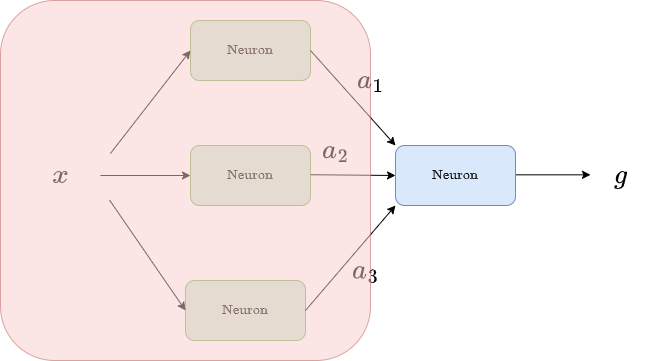
\includegraphics[width=80mm,scale=0.4]{images/nn_images/abstracting_A.png}
            \caption*{We can take this entire layer...}
        \end{figure}
        
        \begin{figure}[H]
            \centering
            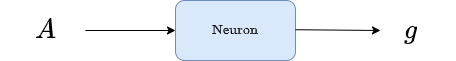
\includegraphics[width=80mm,scale=0.4]{images/nn_images/second_layer.png}
            \caption*{And just reduce it down to the vector $A$.}
        \end{figure}

        Because it's so useful, we'll give this set of neurons a name: a \textbf{layer}.\\
        
        \begin{definition}
            A \vocab{layer} is a set of \gren{neurons} that are in "parallel":
            \begin{itemize}
                \item They all have \gren{inputs} from the same \purp{previous layer}
                    \begin{itemize}
                        \item This \purp{previous layer} could also be the \gren{original input} $x$.
                    \end{itemize}
                
                \item They all have \gren{outputs} to the same \purp{next layer}
                    \begin{itemize}
                        \item This \purp{next layer} could also be the \gren{final output} of the neural network.
                    \end{itemize}
                
                \item And none of these neurons are directly \purp{connected} to each other.
            \end{itemize}
        \end{definition}
        
        This \textbf{layering} structure allows us to simplify our \textbf{analysis}: anything that comes after the layer only has to work with a \textbf{single vector}.
        
        A layer in general might looks like this:
        
        \begin{figure}[H]
            \centering
            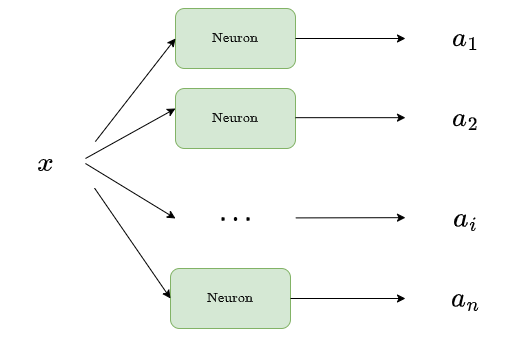
\includegraphics[width=80mm,scale=0.4]{images/nn_images/general_layer.png}
            \caption*{A general layer in a neural network.}
        \end{figure}
        
    \subsection{The Basic Structure of a Neural Network}
        
        We could pick many structures for neural networks, but for simplicity, this will define our \textbf{template} for this chapter.\\
        
        \begin{definition}
            We structure our \vocab{neural networks} as a series of \purp{layers}, where each layer is the \gren{input} to the next layer.
            
            This means that \purp{layers} are a basic unit of a neural network, one level above a \gren{neuron}.
        \end{definition}
        
        In short, we have:
        
        \begin{itemize}
            \item A \vocab{neuron}, made of a linear and an activation component
            
            \item A \vocab{layer}, made of many neurons in parallel
            
            \item A \vocab{neural} network, made of many layers in series
        \end{itemize}
        
        Our goal is some kind of structure that looks something like this:
        
        \begin{figure}[H]
            \centering
            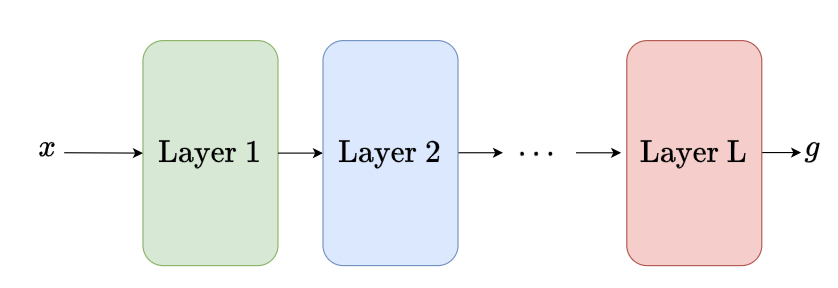
\includegraphics[width=100mm,scale=0.4]{images/nn_images/layers.png}
            \caption*{A neural network.}
        \end{figure}
        
        We now have a high-level view of our entire neural network, so now we dig into the details of a single layer.
        
        
    \subsection{Single Layer: Visualizing our Components}
    
        Now, rather than analyzing a single neuron, we will analyze a single \textbf{layer}.
        
        \begin{figure}[H]
            \centering
            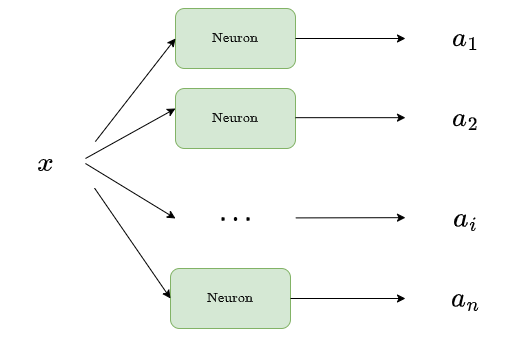
\includegraphics[width=80mm,scale=0.4]{images/nn_images/general_layer.png}
            \caption*{Our first layer.}
        \end{figure}
        
        In order to \textbf{analyze} this layer, we have to open back up the \textbf{abstraction}:
        
        \begin{figure}[H]
            \centering
            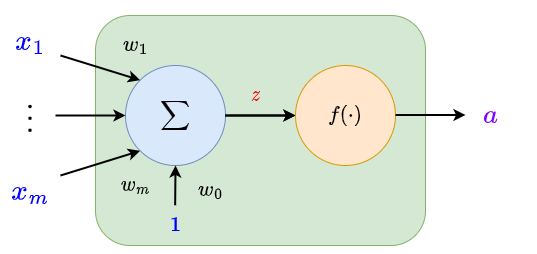
\includegraphics[width=80mm,scale=0.4]{images/nn_images/neuron_inside.png}
            \caption*{Each of those neurons looks like this.}
        \end{figure}
        
        There are two important pieces of \textbf{information} we're hiding:
        
        \begin{itemize}
            \item We have two components inside of our neuron.
            
            \item We have many inputs $x_i$ for one neuron.
        \end{itemize}
        
        The first piece of information is easier to visualize: we just replace each neuron with the two components.
        
        \begin{figure}[H]
            \centering
            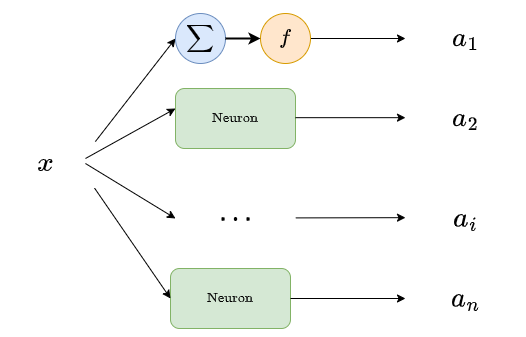
\includegraphics[width=80mm,scale=0.4]{images/nn_images/replace_one_neuron.png}
            \caption*{Replacing one neuron...}
        \end{figure}
        
        \begin{figure}[H]
            \centering
            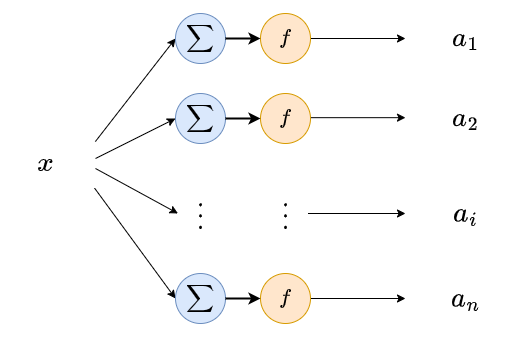
\includegraphics[width=80mm,scale=0.4]{images/nn_images/replace_all_neurons.png}
            \caption*{Replacing all neurons!}
        \end{figure}
    
    \subsection{Single Layer: Visualizing our Inputs}
    
        The second piece of information is much more difficult: we show all of the $x_i$ outputs.
        
        \begin{figure}[H]
            \centering
            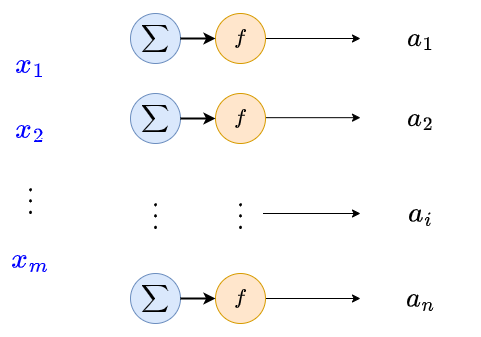
\includegraphics[width=80mm,scale=0.4]{images/nn_images/layers_with_input.png}
        \end{figure}
        
        Now we have to draw the arrow for each input.
        
        \begin{figure}[H]
            \centering
            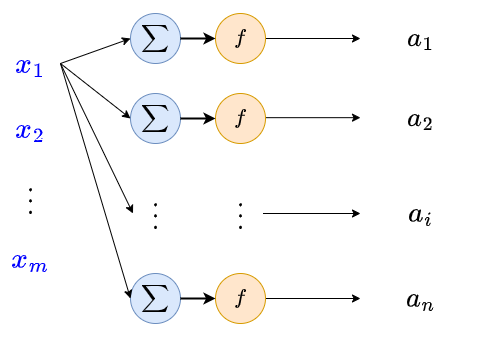
\includegraphics[width=80mm,scale=0.4]{images/nn_images/layers_one_neuron_input.png}
            \caption*{Every neuron receives the first input.}
        \end{figure}
        
        \begin{figure}[H]
            \centering
            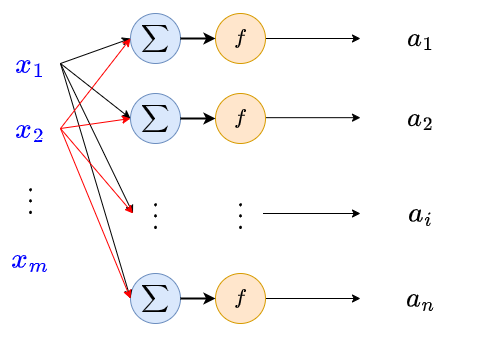
\includegraphics[width=80mm,scale=0.4]{images/nn_images/layers_two_neuron_input.png}
            \caption*{Every neuron receives the second input, too. This is getting messy...}
        \end{figure}
        
        \begin{figure}[H]
            \centering
            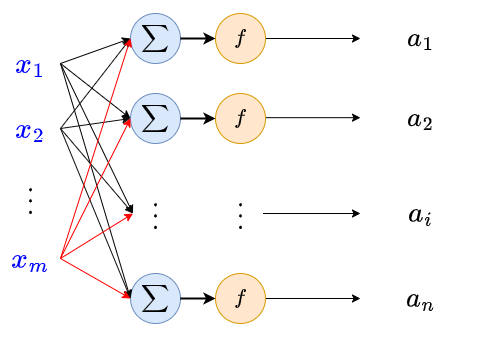
\includegraphics[width=80mm,scale=0.4]{images/nn_images/layers_all_neuron_input.png}
            \caption*{The completed version: this is hard to look at.}
        \end{figure}
        
        Don't worry if this looks \textbf{confusing}! It's natural for it to be \textbf{hard} to read: the only thing you need to know is that we pair \textbf{every} input with \textbf{every} neuron.
        
        This is our \textbf{final} view of this layer: because each of our $m$ inputs has to go to every of $n$ neurons, we end up with $mn$ different \textbf{weights}.
        
        This is a ton of \textbf{information}, and its only one layer! This shows how \textbf{complex} a neural network can be, just by \textbf{combining} simple neurons.
        
        Note that this is a \textbf{fully connected} network: not all networks are FC.\\
        
        \begin{definition}
            A layer is \vocab{fully connected} if every neuron has the \purp{same input vector}.
        \end{definition}
        
        \miniex If one of our neurons \textbf{ignored} $x_1$, but the others did \textbf{not}, the layer would not be \textbf{fully connected}.
        
    \subsection{Dimensions of a layer}
    
        Now that we've seen the \textbf{full} view, we can \textbf{analyze} it. Our goal is to create a more \textbf{useful} and \textbf{accurate} simplification.
        
        Our first point: note that the input and output have a \textbf{different} dimensions!\\
        
        \begin{notation}
            A \vocab{layer} has two associated \purp{dimensions}: the \gren{input} dimension \vocab{$m$} and the \gren{output} dimension \vocab{$n$}.
            
            \begin{itemize}
                \item The \gren{input} dimension \vocab{$m$} is based on the vector output from the \purp{previous layer}: $x \in \RR^m$
                
                \item The \gren{output} dimension \vocab{$n$} is equal to the \purp{number of neurons} in the \gren{current} layer: $A \in \RR^n$
            \end{itemize}
        \end{notation}
        
        \miniex Suppose you have an \textbf{input} vector $x=[x_1, x_2, x_3]$ and two \textbf{neurons}. The dimensions are $m=3$, and $n=2$.
    
        \begin{figure}[H]
            \centering
            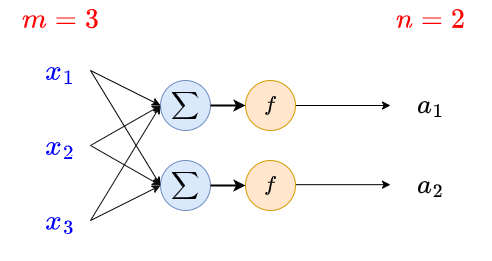
\includegraphics[width=80mm,scale=0.4]{images/nn_images/dimensions_network.png}
            \caption*{The input dimension and output dimensions are \textbf{separate}.}
        \end{figure}
        
    \subsection{The known objects of our layer}
    
        So, we know we have two objects so far:
        
        \begin{itemize}
            \item Our \textbf{input} vector $x \in \RR^m$
            
            \item Our \textbf{output} vector $A \in \RR_n$

        \end{itemize}
        
        Where they each take the form
        
        \begin{equation}
            x = 
                \begin{bmatrix}
                  x_1\\x_2\\ \vdots \\ x_m
                \end{bmatrix}
            \qquad \qquad \qquad
            A =
            \begin{bmatrix}
                a_1\\a_2\\ \vdots \\ a_n
            \end{bmatrix}
        \end{equation}
        
        But, there are a couple other things we haven't \textbf{generalized} for our entire \textbf{layer}:
        
        \begin{itemize}
            \item Our weights 
            \item Our offsets
            \item Our preactivation
        \end{itemize}
        
        \subsection{The other variables of our layer: weights and offsets}
        
        First, our \textbf{weights}: each neuron has its own vector of weights $w \in \RR^m$.
            \note{The dimension needs to match $x$ so we can compute $w^Tx$.}
            
        \begin{equation}
            w = 
            \begin{bmatrix}
              w_1\\w_2\\ \vdots \\ w_m
            \end{bmatrix}
        \end{equation}
        
        To distinguish them from each other, we'll represent the $\nth{i}$ neuron's weights as $\vec{w}_i$.
        
        \begin{equation}
            \vec{w}_i = 
            \begin{bmatrix}
              w_{1i}\\w_{2i}\\ \vdots \\ w_{mi}
            \end{bmatrix}
        \end{equation}
            
        Each needs to be used to \textbf{compute} $a_i$, but having so many objects is annoying.
        
        Remember that, when we had \textbf{multiple} data points $\exi$, we worked with them at the \textbf{same time} by stacking them in a \textbf{matrix}. Let's do the same here:
        
        \begin{equation}
            W = 
            \overbrace{
                \begin{bmatrix}
                  \vec{w}_1 & \vec{w}_2 & \cdots & \vec{w}_n
                \end{bmatrix}
            }^{\text{Each neuron has a weight vector}}
        \end{equation}
        
        If we expand it out, we get a full matrix...
        
        \begin{equation}
            W = 
            \overbrace{
                \begin{bmatrix}
                  w_{\red{11}} & w_{\red{12}} & \cdots & w_{\red{1n}} \\
                  w_{\red{21}} & w_{\red{22}} & \cdots & w_{\red{2n}} \\
                  \vdot        & \vdots       & \ddots & \vdots \\
                  w_{\red{m1}} & w_{\red{m1}} & \cdots & w_{\red{mn}} \\
                \end{bmatrix}
            }^{\red{n} \text{ neurons}}
            \bigggrB{70pt} \red{m} \text{ inputs}
        \end{equation}
        
        This is our \textbf{weight matrix} $W$: it's an $(m \times n)$ matrix. It contains all of our $mn$ weights, sorted by
        
        \begin{itemize}
            \item \vocab{Input variable} (row)
            \item \vocab{Neuron} (column)
        \end{itemize} 
        
        We can do this for our \textbf{offsets} too: thankfully, there is only \textbf{one} offset per neuron, so we can write:
        
        \begin{equation}
            W_0 = 
                \begin{bmatrix}
                  w_{\red{01}} \\ w_{\red{02}} \\ \vdots \\ w_{\red{0n}}
                \end{bmatrix}
            \bigggrB{70pt} \text{Each neuron has an offset}
        \end{equation}
        
        This is our offset vector, with the shape $(n \times 1)$.\\
        
        \begin{notation}
            We can store our \vocab{weights} and \vocab{offsets} as \purp{matrices}:
            
            \begin{itemize}
                \item \purp{Weight} matrix $W$ has the shape $\blu{(m \times n)}$
                
                \item \purp{Offset} matrix $W_0$ has the shape $\blu{(n \times 1)}$
            \end{itemize}
        \end{notation}
        
        These matrices give us a tidy way to understand all of this mess:
        
        \begin{figure}[H]
            \centering
            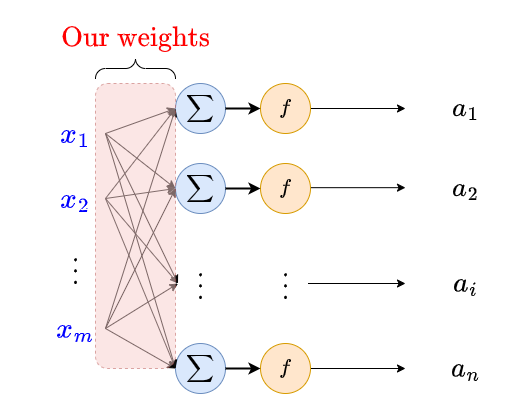
\includegraphics[width=80mm,scale=0.4]{images/nn_images/weights_highlighted.png}
        \end{figure}
        
        Now that we understand it, we'll \textbf{hide} those weights again, for readability.
        
        \begin{figure}[H]
            \centering
            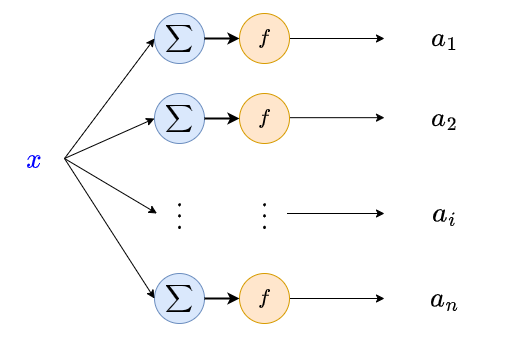
\includegraphics[width=80mm,scale=0.4]{images/nn_images/remove_input.png}
        \end{figure}
        
    
    \subsection{Pre-activation}
    
        Now, all that remains is the pre-activation $z$.
        
        Before, we did 
        
        \begin{equation}
            w^Tx + w_0 = z
        \end{equation}
        
        Because we so carefully kept our weights and offsets separate, we can still do this!
        
        \begin{equation}
            W^Tx + W_0 = Z
        \end{equation}
        
        This pre-activation vector $Z$ contains all of the outputs of our linear components:
        
        \begin{equation}
            Z = 
            \begin{bmatrix}
              z_1 \\ z_2 \\ \vdots \\ z_n
            \end{bmatrix}
        \end{equation}
        
        On our diagram, we can see it here:
        
        \begin{figure}[H]
            \centering
            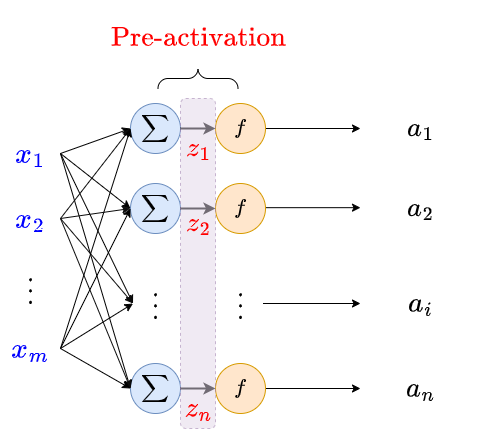
\includegraphics[width=80mm,scale=0.4]{images/nn_images/pre_activation.png}
            \caption*{This section is what $Z$ details with.}
        \end{figure}
        
        And we can connect this to our activation: each $a_i$ is the result of running our function $f$ on $z_i$:
            \note{Because we run the function on each element in $Z$, we call this an \textbf{element-wise} use of our function.}
        
        \begin{equation}
            A = 
            \red{f}(Z)=
            \begin{bmatrix}
              \red{f}(z_1) \\ \red{f}(z_2) \\ \vdots \\ \red{f}(z_n)
            \end{bmatrix}
        \end{equation}
        
    \subsection{Summary of layer}
    
        So, we can now break our our layer up into pieces:\\
        
        \begin{notation}
            Our \vocab{layer} is a \purp{function} that takes in $x \in \RR^m$, and returns $A \in \RR^n$.
            
            It is defined by:
            
            \begin{itemize}
                \item \vocab{Dimensions}: $m$ for \gren{input}, $n$ for \gren{output} (number of neurons)
            \end{itemize}
            
            And our different \purp{matrices}:
            
            \begin{itemize}
                \item \vocab{Input}: a \purp{column vector} $X$ in the shape $(\blu{m} \times 1)$
            
                \item \vocab{Weights}: a \purp{matrix} $W$ in the shape $(\blu{m} \times \red{n})$
                
                \item \vocab{Offset}: a \purp{column vector} $W_0$ in the shape $(\red{n} \times 1)$
                
                \item \vocab{Pre-activation}: a \purp{column vector} $Z$ in the shape $(\red{n} \times 1)$
                
                \item \vocab{Activation}: a \purp{column vector} $A$ in the shape $(\red{n} \times 1)$
            \end{itemize}
        \end{notation}
        
        We've now accomplished our goal: \textbf{simplify} the layer into its \textbf{base} components, without losing any crucial \textbf{information}.
        
        We've can represent an entire layer like this:
        
        \begin{figure}[H]
            \centering
            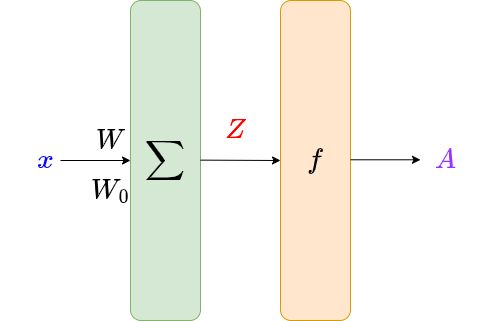
\includegraphics[width=100mm,scale=0.4]{images/nn_images/layer_simplified.png}
        \end{figure}
        
        Note how similar this looks to a \textbf{single} neuron: this works because the neurons in a \textbf{layer} are in \textbf{parallel}!
        
        \begin{figure}[H]
            \centering
            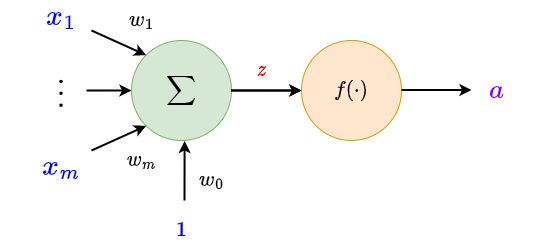
\includegraphics[width=100mm,scale=0.4]{images/nn_images/full_neuron.png}
        \end{figure}
        
        The math is very similar as well:\\
        
        \begin{definition}
            Our \vocab{layer} can be represented by
            
            \begin{itemize}
                \item A \vocab{linear} component that takes in $x$, and outputs \purp{pre-activation} $Z$:
                
                \begin{equation*}
                    Z = W^T x + W_0
                \end{equation*}
                
                \item A (potentially nonlinear) \vocab{activation} component that takes in $Z$, and outputs \purp{activation} $A$:
                
                \begin{equation*}
                    A = f(Z)
                \end{equation*}
                
            \end{itemize}
        
            When we \purp{compose} them together, we get
                
                \begin{equation*}
                    A = f(Z) = f \Big( W^Tx+W_0 \Big)
                \end{equation*}
        \end{definition}
        
    \subsection{The weakness of a single layer}
    
        What can we do with a single layer? Well, our \textbf{LLC} model gives us an example: it has the \textbf{nonlinear} sigmoid activation, but acts as a \textbf{linear} separator.
        
        Why is that? Why is the separator still linear, if the \textbf{activation} isn't?
        
        Well, let's take the \textbf{linear} separator created by the pre-activation:
        
        \begin{equation}
            z = w^T x + w_0 = 0 
        \end{equation}
        
        This is our \textbf{boundary} for just a linear function. But adding the nonlinear activation should make it more \textbf{complex}, right? 
        
        Well, it turns out, we can represent our \textbf{activation} boundary with a \textbf{linear} boundary.
        
        \miniex Continue our LLC example. If $z=0$, then $\sigma(z) = \sigma(0)$. Our boundary is
        
        \begin{equation}
            \sigma(z)=\sigma(0)=\frac{1}{2}
        \end{equation}
        
        Wait. But that means that $\sigma(z)=.5$ is the same as $z=0$: the same inputs $x$ cause both of them, so they have the same boundary!
        
        \begin{equation}
            \text{Linear boundary } z=0 \Longleftrightarrow f(z)=\frac{1}{2}
        \end{equation}
        
        Summary:
        
        \begin{itemize}
            \item $\sigma(z)=.5$ is the \textbf{same} as $z=0$.
            \item $z=0$ is \textbf{linear}.
            \item Thus, our sigmoid boundary is \textbf{linear}.
        \end{itemize}
        
        We can apply this to other activation functions. In general, any constant boundary for most $f(z)$ is equivalent to some linear boundary $z=C$:
            \note{Assuming that $f$ is invertible, which it often is.}
        
        \begin{equation}
            z=C 
            \qquad
            \Longleftrightarrow
            \qquad
            f(z)=f(C)
        \end{equation}
        
        Since $z=C$ is linear, we know that our activation separator $f(x)=f(C)$ is linear too.\\
        
        \begin{concept}
            A single neuron creates a \vocab{linear separator}, even if it has a \purp{nonlinear} activation.
            
            This is because any \gren{boundary} for $f(z)$ we can create, can be represented by some \purp{linear} boundary in $z$.
        \end{concept}
        
            \note{There are exceptions, but this is true for most useful activation functions.}
        
        It turns out, adding more neurons \textbf{within} the layer doesn't change much: because they act in \textbf{parallel}, each neuron acts separately, and the things we said above are still \textbf{true} for each output $a_i$.
        
        \begin{figure}[H]
            \centering
            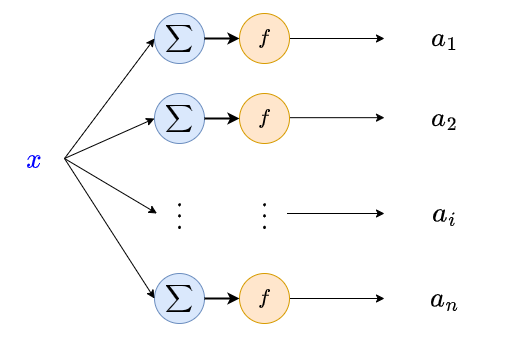
\includegraphics[width=80mm,scale=0.4]{images/nn_images/remove_input.png}
            \caption*{Each of these neurons has the same input, $x$.}
        \end{figure}
        
        So, in order to create nonlinear behavior, we need at least two layers of neurons in \textbf{series}.
        
        So, we'll start \textbf{stacking} layers on each other: each layer \textbf{feeds} into the next one.\\
        
        \begin{concept}
            A \vocab{single layer} of neurons has \gren{linear} behavior.
            
            We need \gren{multiple} layers to get a nonlinear \purp{neural network}.
        \end{concept}
    
    \subsection{Adding a second layer}
    
        So, let's add one more \textbf{layer}. We'll label layers by using a \textbf{superscript}: $W^1$ is the set of \textbf{weights} for the \textbf{first} layer, for example.
        
        \begin{figure}[H]
            \centering
            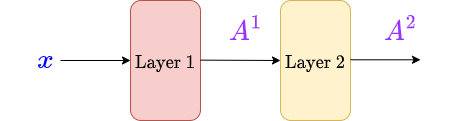
\includegraphics[width=100mm,scale=0.4]{images/nn_images/two_layers.png}
            \caption*{We have two separate outputs: $A^1$ and $A^2$.}
        \end{figure}
        
        \begin{clarification}
            \vocab{Superscripts} in our notation indicate the \purp{layer} that our value is associated with.
            
            They do \purp{not} represent exponentiation! 
        \end{clarification}
        
        \miniex $Z^3$ would be the \textbf{pre-activation} for layer 3: it is \textbf{not} Z "cubed".
        
        What can we learn from this?
        
        \begin{itemize}
            \item The \textbf{output} of layer 1, $A^1$, is the \textbf{input} to layer 2.
            
            \item Thus, the output dimension $n^1$ of layer 1 must \textbf{match} the input $m^2$ of layer 2: 
            
            \begin{equation}
                n^1=m^2
            \end{equation}
        \end{itemize}
        
        Let's break these into their components again.
        
        \begin{figure}[H]
            \centering
            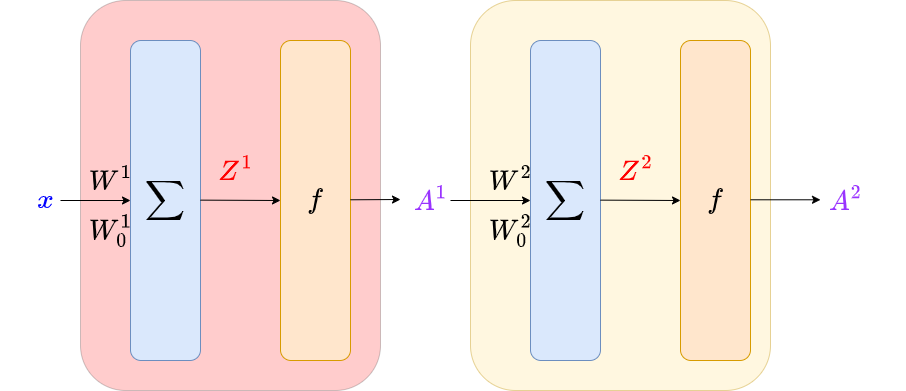
\includegraphics[width=100mm,scale=0.4]{images/nn_images/two_layers_internal.png}
            \caption*{We have two separate outputs: $A^1$ and $A^2$.}
        \end{figure}
        
        To distinguish between the linear functions in each layer, we'll just notate them using the weights and offsets.
        
        \begin{figure}[H]
            \centering
            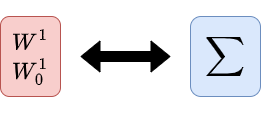
\includegraphics[width=40mm,scale=0.4]{images/nn_images/linear_module_representation.png}
            \caption*{These two are equivalent (if in the same layer)! We'll use the notation on the left, so that you know which layer our unit is in.}
        \end{figure}
        
        And this gives us:
        
        \begin{figure}[H]
            \centering
            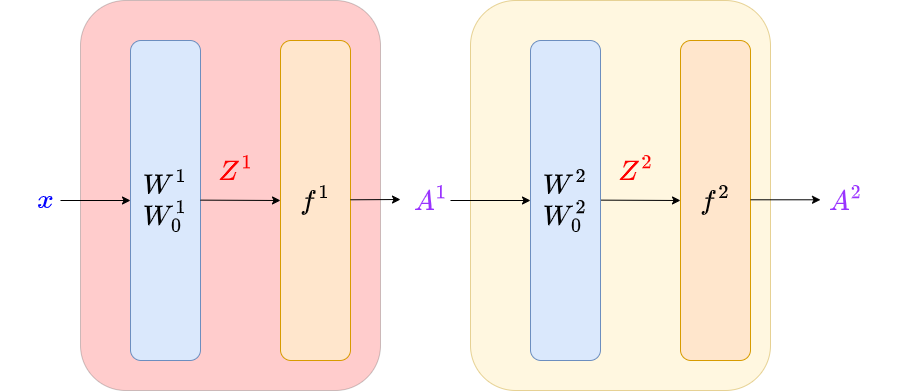
\includegraphics[width=100mm,scale=0.4]{images/nn_images/two_layer_new_notation.png}
        \end{figure}
        
        Now, we can make our functions. For layer one:
        
        \begin{equation}
            \red{A^1} = f(Z^1) = 
            f  
            \Big( 
                (\red{W^1})^T x + \red{W_0^1} 
            \Big)
        \end{equation}
        
        And layer two:
        
        \begin{equation}
            \blu{A^2} = f(Z^2) = 
            f  
            \Big( 
                (\blu{W^2})^T \red{A^1} + \blu{W_0^2} 
            \Big)
        \end{equation}
        
        We can use this to build our \textbf{general} pattern.
        
    \subsection{Many Layers}
    
        We are finally ready to build our \textbf{complete} neural network. We'll just retrace the steps of the 2-layer case.\\
        
        \begin{notation}
            The total \purp{number} of \vocab{layers} in our \vocab{neural network} is notated as $L$.
            
            Typically we notate an \purp{arbitrary} layer as $\ell$ (or $l$).
        \end{notation}
        
        Since $x$ is, for all purposes, \textbf{equivalent} to a vector $A$, we will call it $A^0$.\\
        
        \begin{notation}
            Our \vocab{neural network}'s input $x$ is used in the \gren{same} way as every term $A^\ell$.
            
            So, we will \purp{represent} it as 
            
            \begin{equation*}
                x = A^0
            \end{equation*}
        \end{notation}
        
        \begin{figure}[H]
            \centering
            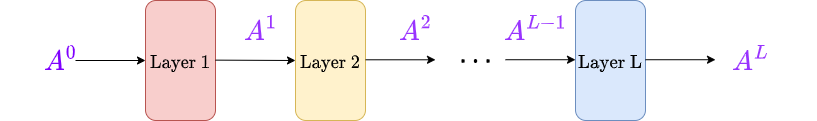
\includegraphics[width=140mm,scale=0.4]{images/nn_images/all_layers.png}
        \end{figure}
        
        Again, we see that the \textbf{output} of layer $\ell$ is the \textbf{input} of layer $\ell+1$.\\
        
        \begin{concept}
            Each layer \vocab{feeds} into the next layer.
            
            $A^\ell$ is the \purp{output} of layer $\ell$, and the \purp{input} of layer $\ell+1$.
            
            This means that the \purp{output} dimension must \gren{match} the next \purp{input} dimension.
            
            \begin{equation*}
                \overbrace{
                    n^\ell
                }^{\text{Output}}
                =
                \overbrace{
                    m^{\ell+1}
                }^{\text{Output}}
            \end{equation*}
            
            And the \vocab{dimension} of $A^\ell$ is $(n^\ell \times 1) = (m^{\ell+1} \times 1)$.
        \end{concept}
        
    \subsection{Our Complete Neural Network}
    
        We can break our layers into components, so we can see the functions involved. 
        
        With this, we build our final neural network:
        
        \begin{figure}[H]
            \centering
            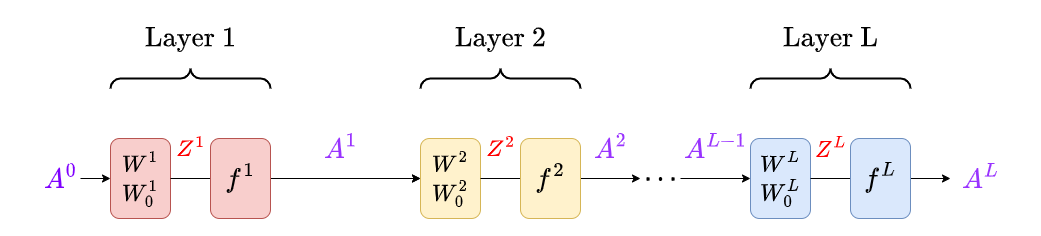
\includegraphics[width=140mm,scale=0.4]{images/nn_images/final_neural_network.png}
        \end{figure}
        
        With this, we can see how each layer is \textbf{related} to each other: as we \textbf{mentioned}, the \textbf{output} of one layer is the \textbf{input} of the next layer.
        
        Here is the computation we do for layer $\ell$:\\
        
        \begin{kequation}
            The calculations done by layer $\ell$ are given by
            
            \begin{equation*}
                \blu{Z^\ell} = (\blu{W^\ell})^T \red{A^{\ell-1}} + \blu{W_0^\ell} 
            \end{equation*}
            
            and
            
            \begin{equation*}
                \blu{A^\ell} = f(\blu{Z^\ell})
            \end{equation*}
            
            Which combine into:
            
            \begin{equation*}
                \blu{A^\ell} = f(\blu{Z^\ell}) = 
                f  
                \Bigg( 
                    (\blu{W^\ell})^T \red{A^{\ell-1}} + \blu{W_0^\ell} 
                \Bigg)
            \end{equation*}
        \end{kequation}
        
        
    
%\pagebreak
%%%%%%%%%%%%%%%%%%%%%%%%%%%%%%%%%%%%%%%%%%%%%%%%%%%%%%%%%%%%%%%%%%%%%%%%%%%%%  
\section{Choices of activation function (WIP)}
%\pagebreak
%%%%%%%%%%%%%%%%%%%%%%%%%%%%%%%%%%%%%%%%%%%%%%%%%%%%%%%%%%%%%%%%%%%%%%%%%%%%%  
\section{Loss functions and activation functions (WIP)}
%\pagebreak
%%%%%%%%%%%%%%%%%%%%%%%%%%%%%%%%%%%%%%%%%%%%%%%%%%%%%%%%%%%%%%%%%%%%%%%%%%%%%  
\section{Error back-propagation (WIP)}
%\pagebreak
%%%%%%%%%%%%%%%%%%%%%%%%%%%%%%%%%%%%%%%%%%%%%%%%%%%%%%%%%%%%%%%%%%%%%%%%%%%%%  
\section{Training (WIP)}
%\pagebreak
%%%%%%%%%%%%%%%%%%%%%%%%%%%%%%%%%%%%%%%%%%%%%%%%%%%%%%%%%%%%%%%%%%%%%%%%%%%%%  

\section{Old Materials}



\section{Networks}


%\pagebreak
%%%%%%%%%%%%%%%%%%%%%%%%%%%%%%%%%%%%%%%%%%%%%%%%%%%%%%%%%%%%%%%%%%%%%%%%%%%%%  

\section{Choices of activation function}

There are many possible choices for the activation function.  We will
start by thinking about whether it's really necessary to have an $f$
at all.

What happens if we let $f$ be the identity?  Then, in a network with
$L$ layers (we'll leave out $W_0$ for simplicity, but keeping it
wouldn't change the form of this argument), 
\[A^L = {W^L}^T A^{L-1} = 
 {W^L}^T {W^{L-1}}^T \cdots {W^1}^T X\;\;.\]
So, multiplying out the weight matrices, we find that 
\[A^L = W^\text{total}X\;\;,\]
which is a {\em linear} function of $X$!
Having all those layers did not change the representational
capacity of the network: the non-linearity of the activation function
is crucial.
\question{Convince yourself that any function representable by any
  number of linear layers (where $f$ is the identity function) can be
  represented by a single layer.}

Now that we are convinced we need a non-linear activation, let's
examine a few common choices.
\begin{description}
  \item{\bf Step function:} 
    $$\text{step}(z) =
    \begin{cases}
      0 & \text{if $z<0$}\\
      1 & \text{otherwise}
    \end{cases}$$
  \item{\bf Rectified linear unit (ReLU):} 
    $$\text{ReLU}(z) =
    \begin{cases}
      0 & \text{if $z<0$}\\
      z & \text{otherwise}
    \end{cases} = \max(0,z)$$ 
  \item{\bf Sigmoid function:} Also known as a {\em logistic} function, can
    be interpreted as probability, because for any value of $z$ the
    output is in $(0, 1)$
    $$\sigma(z) = \frac{1}{1+e^{-z}}$$
  \item{\bf Hyperbolic tangent:} Always in the range $(-1, 1)$
 $$\tanh(z) = \frac{e^z - e^{-z}}{e^z + e^{-z}}$$
\item{\bf Softmax function:}
Takes a whole vector $Z \in \R^n$ and generates as output a vector
$A \in (0, 1)^n$ with the property that $\sum_{i = 1}^n A_i = 1$,
which means we can interpret it as a probability distribution over $n$ items:
\[\text{softmax}(z) =
  \begin{bmatrix}
    \exp(z_1) / \sum_{i} \exp(z_i) \\
    \vdots \\
    \exp(z_n) / \sum_{i} \exp(z_i)
\end{bmatrix}\]

\end{description}

\begin{center}
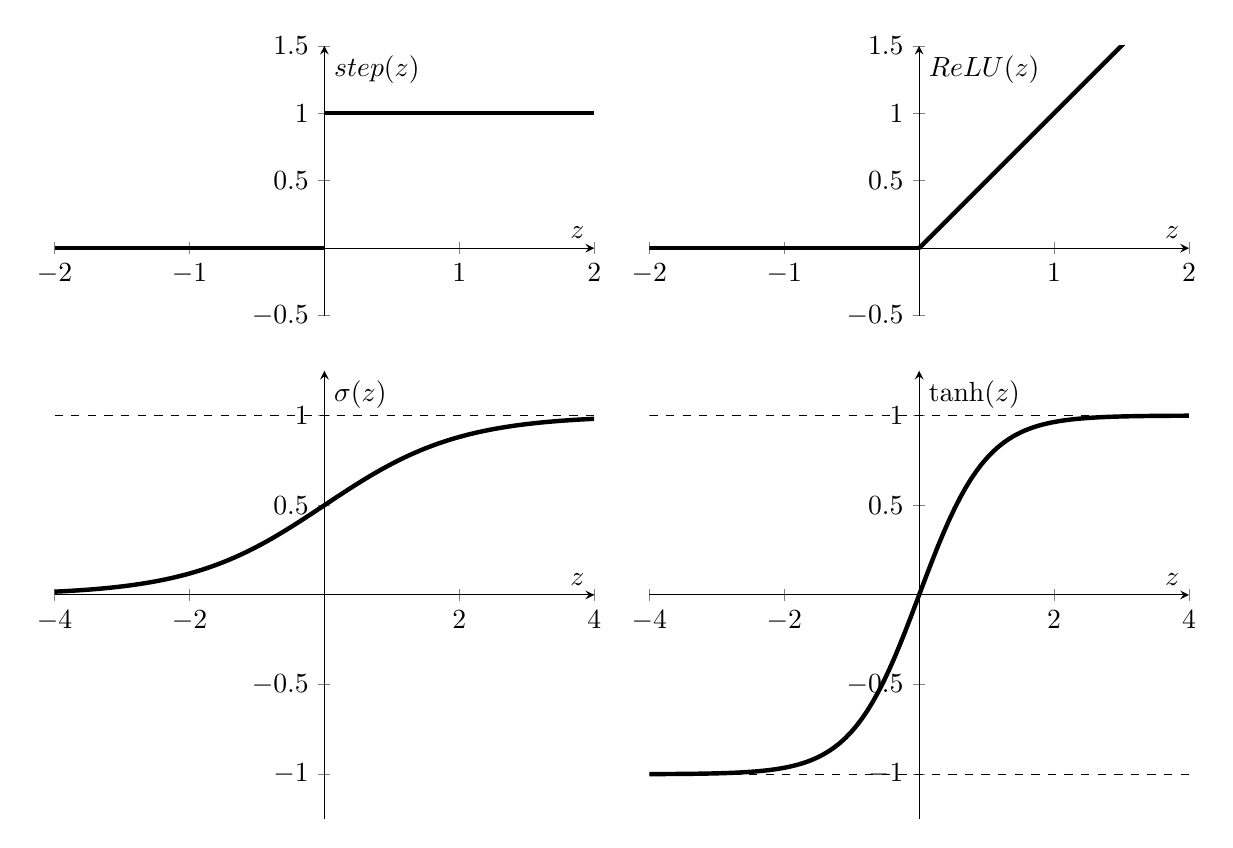
\begin{tikzpicture}
\begin{axis}[
    name=topleft,
    axis lines=middle, axis equal image,
    xmin=-2, xmax=2,
    ymin=-.5, ymax=1.5,
    xlabel={$z$}, ylabel={$\text{step}(z)$},
]
\addplot [domain=-2:0, samples=2, ultra thick] {0}; 
\addplot [domain=0:2, samples=2, ultra thick] {1};
\end{axis}

\begin{axis}[
    name=topright,
    axis lines=middle, axis equal image,
    xmin=-2, xmax=2,
    ymin=-.5, ymax=1.5,
    xlabel={$z$}, ylabel={$\text{ReLU}(z)$},
    at = (topleft.east), anchor=west, xshift=.7cm
]
\addplot [domain=-2:0, samples=2, ultra thick] {0}; 
\addplot [domain=0:2, samples=2, ultra thick] {x};
\end{axis}

\begin{axis}[
    name=bottomleft,
    axis lines=middle, %axis equal image,
    xmin=-4, xmax=4,
    ymin=-1.25, ymax=1.25,
    xlabel={$z$}, ylabel={$\sigma(z)$},
    at = (topleft.south), anchor=north, yshift=-.7cm
]
\addplot [domain=-4:4, samples=100, ultra thick] {1/(1+exp(-x))};
\addplot [domain=-4:4, samples=2, dashed] {1};
\addplot [domain=-4:4, samples=2, dashed] {0};
\end{axis}

\begin{axis}[
    name=bottomright,
    axis lines=middle, %axis equal image,
    xmin=-4, xmax=4,
    ymin=-1.25, ymax=1.25,
    xlabel={$z$}, ylabel={$\tanh(z)$},
    at = (bottomleft.east), anchor=west, xshift=.7cm
]
\addplot [domain=-4:4, samples=100, ultra thick]
  {(exp(x) - exp(-x))/(exp(x) + exp(-x))};
\addplot [domain=-4:4, samples=2, dashed] {1};
\addplot [domain=-4:4, samples=2, dashed] {-1};
\end{axis}
\end{tikzpicture}
\end{center}

The original idea for neural networks involved using the {\bf step}
function as an activation, but because the derivative of the
step function is zero everywhere except at the discontinuity
(and there it is undefined), gradient-descent methods won't be useful
in finding a good setting of the weights, and so we won't
consider them further.  They have been replaced, in a sense, by the
sigmoid, relu, and tanh activation functions.
\question{
Consider sigmoid, relu, and tanh activations.  Which one is most like
a step function?  Is there an additional parameter you could add to a
sigmoid that would make it be more like a step function? 
}
\question{
What is the derivative of the relu function?  Are there some values of
the input for which the derivative vanishes?
}

ReLUs are especially common in internal (``hidden'') layers, and
sigmoid activations are common for the output for binary
classification and softmax for multi-class classification
(see section~\ref{logistic} for an explanation). 

\section{Loss functions and activation functions}
Different loss functions make different assumptions about the range of
inputs they will get as input and, as we have seen, different
activation functions will produce output values in different ranges.
When you are designing a neural network, it's important to make these
things fit together well.  In particular, we will think about matching
loss functions with the activation function in the last layer, $f^L$.  
Here is a table of loss functions and activations that make sense for them:
\begin{center}
\begin{tabular}{c c l}
  Loss & $f^L$ & task\\
  \hline
  squared & linear & regression \\
%  hinge & linear \\
  {\sc nll} & sigmoid & classification\\
  {\sc nllm} & softmax & multi-class classification
\end{tabular}
\end{center}
We explored squared loss in chapter~\ref{chap:regression} and
{\em negative log likelihood} ({\sc nll} and {\sc nllm}) in
chapter~\ref{ch:classification}. 


%\pagebreak
%%%%%%%%%%%%%%%%%%%%%%%%%%%%%%%%%%%%%%%%%%%%%%%%%%%%%%%%%%%%%%%%%%%%%%%%%%%%%  

\section{Error back-propagation}
We will train neural networks using gradient descent methods.  It's
possible to use {\em batch} gradient descent, in which we sum up the
gradient over all the points (as in section~\ref{sec:gd} of
chapter~\ref{chap:gradient}) or
stochastic gradient descent ({\sc sgd}), in which we take a small step with
respect to the gradient considering a single point at a time (as in
section~\ref{sec:sgd} of chapter~\ref{chap:gradient}).

Our notation is going to get pretty hairy pretty quickly.  To keep it
as simple as we can, we'll focus on computing the contribution of one
data point $\ex{x}{i}$ to the gradient of the loss with respect to the
weights, for {\sc sgd}; you can simply sum up these gradients over all
the data points if you wish to do batch descent.

So, to do {\sc sgd} for a training example $(x, y)$, we need to
compute $\nabla_W \text{Loss}(NN(x;W),y)$, 
where $W$ represents all weights $W^l, W_0^l$ in all the layers $l =
(1, \ldots, L)$. This seems terrifying,
but is actually quite easy to do using the chain rule. 
\note{Remember the chain rule!  If $a = f(b)$ and $b = g(c)$ (so that\\
  $a = f(g(c))$), then \\$\frac{d a}{d c} = \frac{d a}{d b} \cdot \frac{d
    b}{d c} = f'(b) g'(c) = f'(g(c)) g'(c)$.}

Remember that we are always computing the gradient of the loss
function {\em with respect to the weights} for a particular value of
$(x,  y)$.  That tells us how much we want to change the weights, in
order to reduce the loss incurred on this particular training example.

First, let's see how the loss depends on the weights in the final
layer, $W^L$.  Remembering that our output is $A^L$, and using the
shorthand $\text{loss}$ to stand for $\text{Loss}((NN(x;W),y)$ which
is equal to $\text{Loss}(A^L, y)$, and finally that $A^L = f^L(Z^L)$ and
$Z^L = {W^L}^T A^{L-1} +W_0^L$, we can use the chain rule, stated informally as:\note{It might reasonably bother you that $\partial{Z^L}/\partial{W^L}
  = A^{L-1}$.  We're somehow thinking about the derivative of a vector
  with respect to a matrix, which seems like it might need to be a
  three-dimensional thing.  But note that
  $\partial{Z^L}/\partial{W^L}$ is really 
  $(\partial{{W^L}^T A^{L-1}})/\partial{W^L}$ and it seems okay in at
  least an informal sense that it's $A^{L-1}$.  See the box below for
  a proof.}
\[
  \frac{\partial \text{loss}}{\partial W^L} = 
  \underbrace{\frac{\partial Z^L}{\partial W^L}}_{\text{$A^{L-1}$}}
\cdot
  \underbrace{\frac{\partial A^L}{\partial Z^L}}_{f^{L'}} 
\cdot
\underbrace{
  \frac{\partial \text{loss}}{\partial A^L}}_{\text{depends on loss
  function}} 
\;\;.\]

\def\bea{\begin{eqnarray}}
\def\eea{\end{eqnarray}}

\begin{examplebox}

Now, why do we indicate above that the derivative of $Z^L$ with
respect to $W^L$ is $A^{L-1}$?  This may seem like a strange result,
because $Z^L$ is a $n\times 1$ vector, whereas $W^L$ is a matrix.

However, this is straightforward to see if we simply write out the
indices of the matrices and vectors involved.  Let $[W]_{ab}$ be the
element of matrix $W$ in row $a$, column $b$, and let $[Z]_c$ be the
$c^{\rm th}$ element of vector $Z$.  Recall the last stage of the
neural network, noting the sizes of the matrices and vectors involved:
%~\\

\hspace*{-20ex}
\begin{tikzpicture}
  \coordinate (x) at (0,0);
  \node[inner sep=0em] (w1) at (1.7,0){~};
  \node (dots) at ($5*(w1)$) {$\cdots$};
  \node[inner sep=0em] (wL) at ($6*(w1)$)
    {\begin{tabular}{c} $W^L$ \\ $W^L_0$\end{tabular}};
  \node[inner sep=1em] (fL) at ($7*(w1)$) {$f^L$};
  \coordinate (y) at ($8*(w1) - (.3,0)$);

  \draw[->] (dots) -- node[above] {$A^{L-1}$} (wL);
  \draw[->] (wL) -- node[above] {$Z^L$} (fL);
  \draw[->] (fL) -- node[above] {$A^L$} (y);

%  \draw [decorate,decoration={brace,mirror,amplitude=10pt}]
%    ($(wL) + (-.4, -.7)$) -- node[yshift=-1.8em] {layer $L$}
%    ($(fL) + (.4,-.7)$);

%   \draw
%     ($(wL) + (-.4, -.7)$) -- node[yshift=-1.8em] {$n\times 1$}
%     ($(fL) + (.4,-.7)$);
  \node (nxo) at ($(wL) + (.8, -0.9)$) {$\color{red} n\times 1$};
  \node (mxo) at ($(wL) + (-.8, -0.9)$) {$\color{red} m\times 1$};
  \node (nxot) at ($(fL) + (.8, -0.9)$) {$\color{red} n\times 1$};
  \node (mxn) at ($(wL) + (0, +0.9)$) {$\color{blue} m\times n$};
  \node (nxou) at ($(fL) + (0, +0.9)$) {$\color{blue} n\times 1$};

  \foreach \point in {wL, fL}{
    \draw ($(\point) + (-.3,-.5)$) rectangle ($(\point) + (.3,.5)$);
  }
\end{tikzpicture}
% \end{center}

% ~\\
\noindent
Since we have that
$
	Z^L = (W^L)^T A^{L-1}
$
then, writing out the explicit elements:
\bea
	\left [Z^L \right]_c &=& \sum_{a=1}^m \left[ (W^L)^T \right]_{ca} \left[ A^{L-1} \right]_a
% \\
%	 &=& \sum_{a=1}^m \left[ W^L \right]_{ac} \left[ A^{L-1} \right]_a
	 = \sum_{a=1}^m \left[ W^L \right]_{ac} \left[ A^{L-1} \right]_a
\,.
\eea

The partial derivative we want, expressed with explicit indices, and using $\delta_{bc}$ being $1$ when $b=c$ and $0$ otherwise, is:
\bea
	\frac{\partial \left[Z^L \right]_c}{\partial \left[W^L\right]_{ab}}
	&=& \frac{\partial }{\partial \left[W^L\right]_{ab}} \sum_{a=1}^m \left[ W^L \right]_{ac} \left[ A^{L-1} \right]_a
\\	&=& \frac{\partial }{\partial \left[W^L\right]_{ac}} \sum_{a=1}^m \left[ W^L \right]_{ac} \left[ A^{L-1} \right]_a \delta_{bc}
%	= \frac{\partial }{\partial \left[W^L\right]_{ac}} \sum_{a=1}^m \left[ W^L \right]_{ac} \left[ A^{L-1} \right]_a \delta_{bc}
\\	&=& \left[ A^{L-1} \right]_a \delta_{bc}
\,.
\eea
The derivative is naturally expected to be zero when the column index
of $W^L$ is unequal to the row index of $Z^L$, because the $c^{\rm
  th}$ column of $W^L$ generates the $c^{\rm th}$ row of $Z^L$.  Thus,
$\partial Z^L / \partial W^L$ only has one free index,
meaning that it is a vector, and we see from this explicit calculation
that it is the $m\times 1$ vector $A^{L-1}$.

\end{examplebox}
  
To actually get  the dimensions to match, we need to write this a bit
more carefully, and note that it is true for any $l$, \note{Definitely
see the matrix derivative appendix for a detailed discussion of these
operations.} including $l =  L$:
\begin{equation}
\label{eq:gradloss}
  \underbrace{\frac{\partial \text{loss}}{\partial W^l}}_{m^l \times n^l}  =  
\underbrace{A^{l-1}}_{m^l \times 1} \;
\underbrace{\left(\frac{\partial \text{loss}}{\partial
                                              Z^l}\right)^T}_{1 \times n^l}
\end{equation}

Yay!  So, in order to find the gradient of the loss with respect to the
weights in the other layers of the network, we just need to be able to
find $\partial \text{loss}/\partial{Z^l}$.  

If we repeatedly apply
the chain rule, we get this expression for the gradient of the loss
with respect to the pre-activation in the first layer, again stated informally as:
\begin{equation}
\label{eq:gradzfirst}
  \frac{\partial \text{loss}}{\partial Z^1} = \underbrace{\underbrace{
  \frac{\partial \text{loss}}{\partial A^L} \cdot
  \frac{\partial A^L}{\partial Z^L} \cdot
  \frac{\partial Z^L}{\partial A^{L-1}} \cdot
  \frac{\partial A^{L-1}}{\partial Z^{L-1}} \cdot \cdots \cdot
  \frac{\partial A^2}{\partial Z^2}}_{\partial \text{loss} / \partial Z^2}
  \cdot \frac{\partial Z^2}{\partial A^1}}
  _{\partial \text{loss} / \partial A^1} \cdot
  \frac{\partial A^1}{\partial Z^1} \;\;.
\end{equation}
This derivation was informal, to show  you the general structure of
the computation.  In fact, to get the dimensions to all work out, we
just have to write it backwards!  Let's first understand more about
these quantities:
\begin{itemize}
\item $\partial \text{loss}/\partial A^L$ is $n^L \times 1$ and
  depends on the particular loss function you are using.
\item $\partial Z^l / \partial A^{l-1}$ is $m^l \times n^l$ and is
  just $W^l$ (you can verify this by computing a single entry
  $\partial Z^l_i / \partial A^{l-1}_j$).
\item $\partial A^l/\partial Z^l$ is $n^l \times n^l$.  It's a little
  tricky to think about.  Each element 
  $a_i^l = f^l(z_i^l)$. \note{We are treating element-wise 
    activation functions here; consideration of activation layers where
    an output $a_i$ depends on multiple $z_j$, such as {\em softmax}, may
    result in a gradient matrix with non-zero off-diagonal elements.}
    This means that $\partial a_i^l / \partial
  z_j^l = 0$ whenever $i \not = j$.  So, the off-diagonal elements of 
  $\partial A^l/\partial Z^l$ are all 0, and the diagonal elements are 
  $\partial a_i^l / \partial  z_i^l = {f^l}'(z_i^l)$.  
\end{itemize}
Now, we can rewrite equation~\ref{eq:gradzfirst} so that the quantities
match up as
\begin{equation}
\label{eq:gradz}
%\frac{\partial \text{loss}}{\partial A^{l-1}} = 
%W^l \cdot 
\frac{\partial \text{loss}}{\partial Z^l} = 
\frac{\partial A^l}{\partial Z^l} \cdot 
W^{l+1} \cdot \frac{\partial A^{l+1}}{\partial Z^{l+1}} \cdot \ldots
W^{L-1} \cdot \frac{\partial A^{L-1}}{\partial Z^{L-1}} \cdot 
W^{L} \cdot \frac{\partial A^{L}}{\partial Z^{L}} \cdot
\frac{\partial \text{loss}}{\partial A^L}
\end{equation}

Using equation~\ref{eq:gradz} to compute $\partial \text{loss}/\partial{Z^l}$
combined with equation~\ref{eq:gradloss}, lets us find the gradient
of the  loss with respect to any of the weight matrices.
\question{Apply the same reasoning to find the gradients of
  $\text{loss}$ with respect to $W_0^l$.}

This general process is called {\em error back-propagation}.  
\note{We could call this 
 ``blame propagation''.  Think of $\text{loss}$ as how mad we
  are about the prediction just made.  Then $\partial
  \text{loss}/ \partial A^L$ is how much we blame $A^L$ for the loss.
  The last module has to take in $\partial \text{loss}/ \partial A^L$
  and compute $\partial \text{loss}/ \partial Z^L$, which is how much
  we blame $Z^L$ for the loss.  The next module (working backwards)
  takes in $\partial \text{loss}/ \partial Z^L$ and computes $\partial
  \text{loss}/ \partial A^{L-1}$.  So every module is accepting its 
  blame for the loss, computing how much of it to allocate to each of
  its inputs, and passing the blame back to them.}
The idea
is that we first do a {\em forward pass} to compute all the $a$ and
$z$ values at all the layers, and finally the actual loss on this
example.  Then, we can work backward and compute the gradient of the
loss with respect to the weights in each layer, starting at layer $L$
and going back to layer 1.  

\begin{center}
\begin{tikzpicture}[scale=.98]
  \coordinate (x) at (0,0);
  \node[inner sep=0em] (w1) at (1.7,0)
    {\begin{tabular}{c} $W^1$ \\ $W^1_0$\end{tabular}};
  \node[inner sep=1em] (f1) at ($2*(w1)$) {$f^1$};
  \node[inner sep=0em] (w2) at ($3*(w1)$)
    {\begin{tabular}{c} $W^2$ \\ $W^2_0$\end{tabular}};
  \node[inner sep=1em] (f2) at ($4*(w1)$) {$f^2$};
  \node (dots) at ($5*(w1)$) {$\cdots$};
  \node[inner sep=0em] (wL) at ($6*(w1)$)
    {\begin{tabular}{c} $W^L$ \\ $W^L_0$\end{tabular}};
  \node[inner sep=1em] (fL) at ($7*(w1)$) {$f^L$};
  \node (loss) at ($8*(w1)$) {Loss};
  \coordinate (y) at ($8*(w1) + (0,1.5)$);

  \draw[->] (x) -- node[above] {$X = A^0$} (w1);
  \draw[->] (w1) -- node[above] {$Z^1$} (f1);
  \draw[->] (f1) -- node[above] {$A^1$} (w2);
  \draw[->] (w2) -- node[above] {$Z^2$} (f2);
  \draw[->] (f2) -- node[above] {$A^2$} (dots);
  \draw[->] (dots) -- node[above] {$A^{L-1}$} (wL);
  \draw[->] (wL) -- node[above] {$Z^L$} (fL);
  \draw[->] (fL) -- node[above] {$A^L$} (loss);
  \draw[->] (y) -- node[right] {$y$} ($(loss)+(0,.65)$);

  %\draw[->,yshift=0.5cm] (loss.west) to [out=150,in=30] (fL.east);
  \foreach \s/\e/\t in {loss/fL/A^L,
                        fL/wL/Z^L,
                        wL/dots/A^{L-1},
                        dots/f2/A^2,
                        f2/w2/Z^2,
                        w2/f1/A^1,
                        f1/w1/Z^1}{
  \path[->] ($(\s.west) - (0,.5)$) edge[out=210,in=-30] node[below]
    {$\frac{\partial \text{loss}}{\partial \t}$}
    ($(\e.east) - (0,.5)$);
  }
  \foreach \point in {w1, f1, w2, f2, wL, fL}{
    \draw ($(\point) + (-.3,-.5)$) rectangle ($(\point) + (.3,.5)$);
  }
  \draw ($(loss) + (-.4,-.5)$) rectangle ($(loss) + (.4,.5)$);
\end{tikzpicture}
\end{center}

If we view our neural network as a sequential composition of modules
(in our work so far, it has been an alternation between a linear
transformation with a weight matrix, and a component-wise application
of a non-linear activation function), then we can define a simple API
for a module that will let us compute the forward and backward passes,
as well as do the necessary weight updates for gradient descent.  Each
module has to provide the following ``methods.''  We are already using
letters $a, x, y, z$ with particular meanings, so here we will use $u$
as the vector input to the module and $v$ as the vector output:
\begin{itemize}
  \item forward: $u \rightarrow v$
  \item backward: $u, v, \partial L /
    \partial v \rightarrow \partial L / \partial u$
  \item weight grad: $u, \partial L / \partial v \rightarrow \partial L
    / \partial W$  only needed for modules that have weights $W$
\end{itemize}
In homework we will ask you to implement these modules for neural
network components, and then use them to construct a network and train
it as described in the next section.


%\pagebreak
%%%%%%%%%%%%%%%%%%%%%%%%%%%%%%%%%%%%%%%%%%%%%%%%%%%%%%%%%%%%%%%%%%%%%%%%%%%%%  

\section{Training}
Here we go!  Here's how to do stochastic gradient descent training on
a feed-forward neural network.   After this pseudo-code, we motivate
the choice of initialization in lines 2 and 3.  The actual
computation of the gradient values (e.g. $\partial\text{loss}/
\partial A^L$) is not directly defined in this code, because we want
to make the structure of the computation clear.
\question{What is $\partial Z^l / \partial W^l$? }
\question{Which terms in the code below depend on $f^L$?}

\begin{codebox}
  \Procname{$\proc{SGD-Neural-Net}(\dataTrain, T, L, (m^1, \ldots,
    m^L), (f^1, \ldots, f^L), \text{Loss})$}
  \li     \For $l \gets 1$ \To $L$
        \Do
  \li        $W_{ij}^l \sim \text{Gaussian}(0, 1/m^l)$
  \li        $W_{0j}^l \sim \text{Gaussian}(0, 1)$
            \End
  \li \For $t \gets 1$ \To $T$
  \li   \Do
          $i \gets \text{random sample from } \{1,\ldots,n\}$
  \li     $A^0 \gets \ex{x}{i}$
  \li     \Comment forward pass to compute the output $A^L$
  \li     \For $l \gets 1$ \To $L$
  \li       \Do
              $Z^l \gets W^{l^T}A^{l-1} + W_0^l$
  \li         $A^l \gets f^l(Z^l)$
            \End
  \li     $\text{loss} \gets \text{Loss}(A^L, \ex{y}{i})$
  \li     \For $l \gets L$ \To 1:
         \Do
  \li       \Comment error back-propagation
  \li       $\partial \text{loss}/\partial A^l \gets$ 	%
            %            m x 1
            {\bf if} $l < L$ 
            {\bf then}
                % dims:          n x 1                    *    m x n
                $\partial Z^{l+1}/\partial A^l \cdot \partial \text{loss}/\partial Z^{l+1} $   
                % dims:  m x n                   *     n x 1
            {\bf else}
                $ \partial \text{loss}/\partial A^L$
  \li       $\partial \text{loss}/\partial Z^l \gets \partial
  A^l/\partial Z^l  \cdot \partial
  \text{loss}/\partial A^l$
  \li       \Comment compute gradient with respect to weights
  \li       $\partial \text{loss}/\partial W^l  \gets        A^{l-1}      \cdot    \left( \partial \text{loss}/\partial Z^l  \right)^T $
  %                           m x n              =            m x 1          *        1 x n
  \li       $\partial \text{loss}/\partial W_0^l \gets       \partial \text{loss}/\partial Z^l $
  %                           1 x n              =                  1 x n
  \li       \Comment stochastic gradient descent update
  \li       $W^l = W^l - \eta(t)\cdot \partial \text{loss}/\partial W^l$
  \li       $W^l_0 = W_0^l - \eta(t)\cdot \partial \text{loss}/\partial W_0^l$
        \End
\end{codebox}

Initializing $W$ is important;  if you do it badly there is a good
chance the neural network training won't work well.  First, it is
important to initialize the weights to random values.  We want
different parts of the network to tend to ``address'' different
aspects of the problem; if they all start at the same weights, the
symmetry will often keep the values from moving in useful directions.
Second, many of our activation functions have (near) zero slope when
the pre-activation $z$ values have large magnitude, so we generally
want to keep the initial weights small so we will be in a situation
where the gradients are non-zero, so that gradient descent will have
some useful signal about which way to go.  

One good general-purpose strategy is to choose each weight at random
from a Gaussian (normal) distribution with mean 0 and standard
deviation $(1/m)$ where $m$ is the number of inputs to the unit.
\question{If the input $x$ to this unit is a vector of 1's, what would
  the expected pre-activation $z$ value be with these initial
  weights?}  We write this choice (where $\sim$ means ``is drawn
randomly from the distribution'')
    \[W^l_{ij} \sim \text{Gaussian}\left(0,
        \frac{1}{m^l}\right)\;\;.\]

It will often turn out (especially for fancier activations and loss
functions) that computing
\[\frac{\partial \text{loss}}{\partial Z^L}\] is easier than computing
\[\frac{\partial \text{loss}}{\partial A^L}\;\;\text{ and }\;\;\frac{\partial A^L}
{\partial Z^L}\;\;.\] 
So, we may instead ask for an 
implementation of a loss function to provide a backward method that
computes $\partial \text{loss}/\partial Z^L$ directly.

%%% Local Variables:
%%% mode: latex
%%% TeX-master: "top"
%%% End:
